\documentclass[12pt,a4paper,bibliography=totocnumbered,listof=totocnumbered]{article}
\usepackage[ngerman]{babel}
\usepackage[utf8]{inputenc}
%\titlespacing{\section}{0pt}{12pt plus 4pt minus 2pt}{-6pt plus 2pt minus 2pt}

% Kopf- und Fusszeile
\renewcommand{\sectionmark}[1]{\markright{#1}}
\renewcommand{\leftmark}{\rightmark}
\pagestyle{fancy}
\lhead{}
\chead{}
\rhead{\thesection\space\contentsname}
\lfoot{Implementierung von Brettspielen am Beispiel ReversiXT -- SS \the\year}
\cfoot{}
\rfoot{\ \linebreak Seite \thepage}
\renewcommand{\headrulewidth}{0.4pt}
\renewcommand{\footrulewidth}{0.4pt}

% Vorspann
\renewcommand{\thesection}{\Roman{section}}
\renewcommand{\theHsection}{\Roman{section}}
\pagenumbering{Roman}

\newcommand{\folgen}[1]{
\ensuremath
#1
}

\newcommand{\MyTitlepage}[5][\empty]{
\thispagestyle{empty}
\begin{center}
	
\includegraphics[scale=0.2]{pics/oth-logo.png}\\
	\vspace*{2cm}
	\Large
	\textbf{Fakultät}\\
	\textbf{Informatik und Mathematik}\\
	\vspace*{2cm}
	\Huge
	\textbf{Projektbericht}\\
	\vspace*{0.5cm}
	\large
	zum Wahlpflichtfach im SS \the\year\\
	\vspace*{1cm}
	\textbf{Implementierung von Brettspielen am Beispiel ReversiXT}\\
	\vspace*{1cm}
	\includegraphics[height=6cm]{#1}
	\vfill
	\normalsize
	%\newcolumntype{x}[1]{>{\raggedleft\arraybackslash\hspace{0pt}}p{#1}}
	\begin{tabular}{rl}%{6cm}p{7.5cm}}
	    \rule{0mm}{5ex}\textbf{Gruppe:} & #2 \\
		\rule{0mm}{5ex}\textbf{Autoren:} & \hspace*{-0.5em}\begin{tabular}[t]{r}#3\end{tabular} \\ 
		\rule{0mm}{5ex}\textbf{Leiter:} & Prof. Dr. rer. nat. Carsten Kern \\ 
		\rule{0mm}{5ex}\textbf{Abgabedatum:} & #4 \\ 
	\end{tabular} 
\end{center}
\pagebreak
}

\begin{document}

% ----------------------------------------------------------------------------------------------------------
% Titelseite
% ----------------------------------------------------------------------------------------------------------
\MyTitlepage[pics/group-image]{01}{
\texttt{benedikt.halbritter@st.oth-regensburg.de}\\
\texttt{markus1.koch@st.oth-regensburg.de}\\
\texttt{iwan.eckert@st.oth-regensburg.de}}
{??.??.\the\year} % FIXME optional: Gruppenlogo als PNG, Pflichtfelder: Gruppe, Authoren durch "\\" getrennt und Abgabedatum eingeben

\setcounter{page}{1} 
% ----------------------------------------------------------------------------------------------------------
% Inhaltsverzeichnis
% ----------------------------------------------------------------------------------------------------------
\tableofcontents
\pagebreak


% ----------------------------------------------------------------------------------------------------------
% Inhalt
% ----------------------------------------------------------------------------------------------------------
% Abstände Überschrift
%\titlespacing{\section}{0pt}{12pt plus 4pt minus 2pt}{6pt plus 2pt minus 2pt}
%\titlespacing{\subsection}{0pt}{12pt plus 4pt minus 2pt}{4pt plus 2pt minus 2pt}
%\titlespacing{\subsubsection}{0pt}{12pt plus 4pt minus 2pt}{2pt plus 2pt minus 2pt}

% Kopfzeile
\renewcommand{\sectionmark}[1]{\markright{#1}}
\renewcommand{\subsectionmark}[1]{}
\renewcommand{\subsubsectionmark}[1]{}
\lhead{Kapitel \thesection}
\rhead{\rightmark}

\onehalfspacing
\renewcommand{\thesection}{\arabic{section}}
\renewcommand{\theHsection}{\arabic{section}}
\setcounter{section}{0}
\pagenumbering{arabic}
\setcounter{page}{1}

% ----------------------------------------------------------------------------------
% Kapitel: Einleitung
% ----------------------------------------------------------------------------------
\section{Einleitung}\label{sec:einleitung}
ReversiXT ist eine Erweiterung des Brettspiels Reversi, welches in den 1880er Jahren vom Engl\"ander Lewis Waterman entwickelt wurde.
Es handelt sich um ein 2-Personen-Spiel, bei dem man ein 8x8 gro"ses Spielfeld hat.
Es werden je zwei Spielsteine in unterscheidbaren Farbe diagonal zueinander mittig auf dem Spielfeld platziert, wie in der Abbildung~\ref{fig:basicgame} zu sehen ist.
Der blaue Spieler beginnt und darf nun auf leere Felder setzen, die ausgehend von diesem Feld in beliebiger Richtung (senkrecht, waagerecht oder diagonal) einen oder mehrere gegnerische Steine zwischen eigenen Steinen einschlie"sen.
Beim durchf\"uhren eines Spielzuges werden die gegnerischen Spielsteine in die eigene Farbe umgef\"arbt.
Die m\"oglichen Startz\"uge wurden in der Grafik mit eingezeichnet.
Gewonnen hat derjenige, der zum Schluss die meisten Steine hat.

\vspace{1em}
\begin{minipage}{\linewidth}
	\centering
	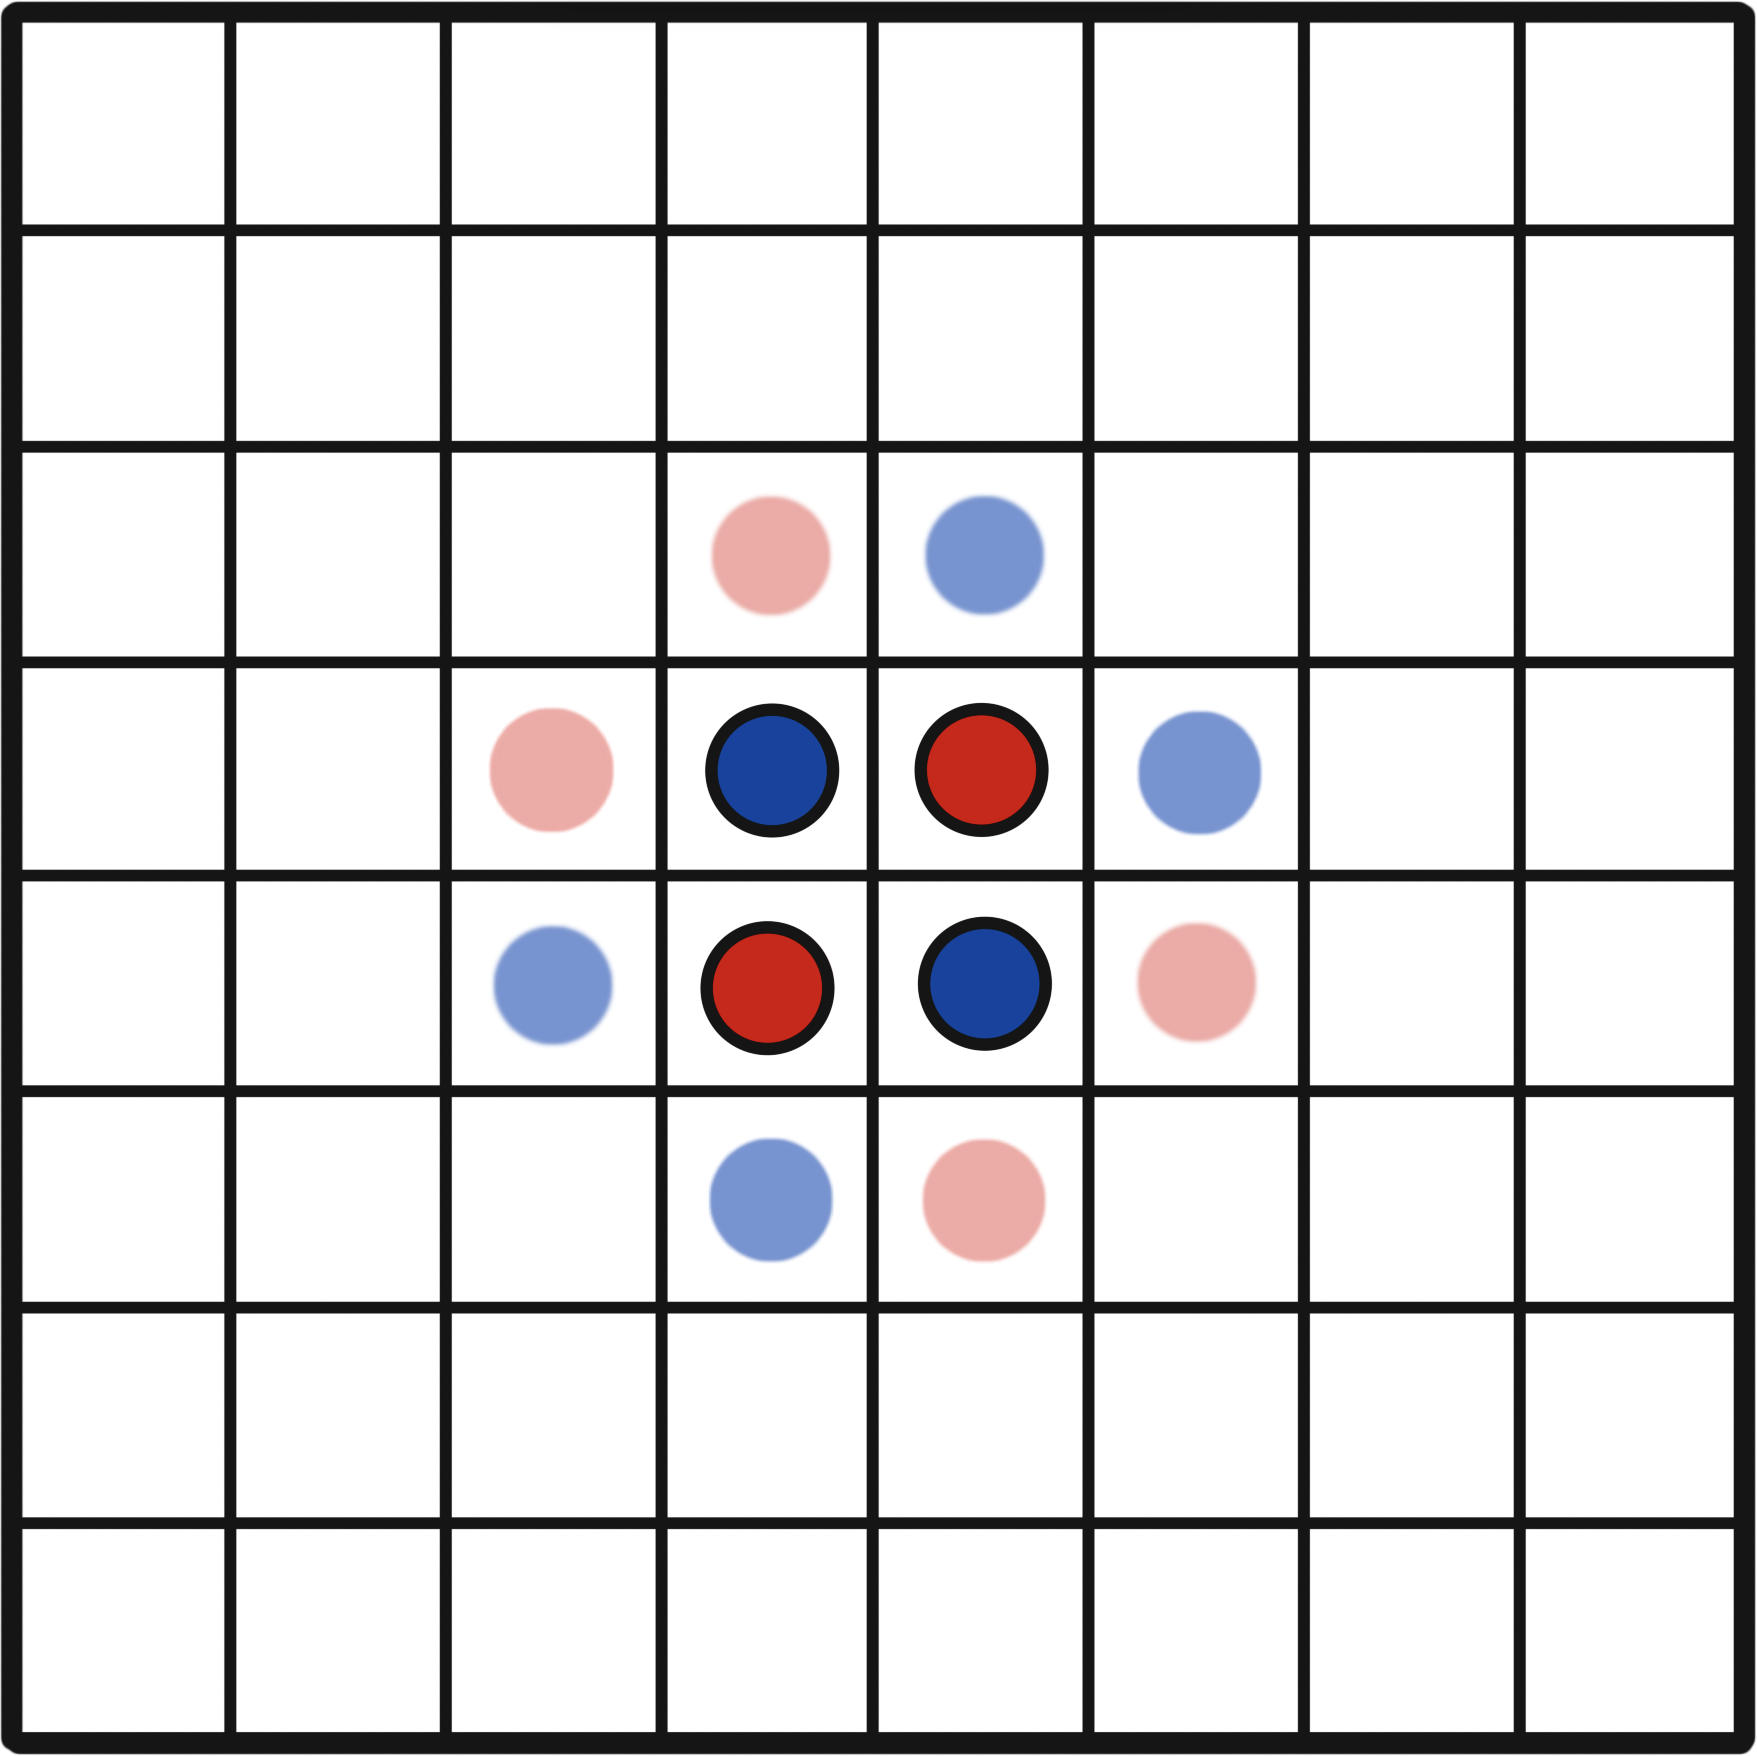
\includegraphics[width=0.5\linewidth]{pics/basicgame-start}
	\captionof{figure}[Grundspiel Start]{Grundspiel Reversi mit möglichen Startzügen}
	\label{fig:basicgame}
\end{minipage}

\subsection{Besonderheiten von ReversiXT}\label{subsec:besonderheiten-von-reversixt}
Das Spiel ReversiXT, was man als Reversi Extreme bezeichnen kann, basiert auf den gleichen Regeln wie das Grundspiel Reversi, hat dabei jedoch einige Zusatzregelungen, welche hier kurz erkl\"art werden.
Bei ReversiXT treten bis zu acht Spieler auf einem maximal 50x50 gro"sen Spielfeld gegeneinander an.
Das Spiel besteht dabei aus zwei unterschiedlichen Spielphasen.
In Phase 1 m\"ussen Spieler solange ziehen, bis keiner mehr kann.
Im Anschluss beginnt die Phase 2, die sogenannte Bombenphase.
Zudem gibt es mehrere Spezialfelder, die vorab fest definiert sind und jeweils nur einmal ausgel\"ost werden k\"onnen.
Mit einem Inversionsfeld werden die Farben aller Spieler um eins verschoben (der letzte Spieler wird zu Spieler 1).
Mit einem Choicefeld wird ein Spieler mit einem Anderen getauscht, hier ist es auch erlaubt sich selbst zu w\"ahlen.
Ein Expansionsfeld wird als Gegner gewertet und kann nach den gleichen Regeln wie andere Spieler eingenommen werden, oder mithilfe eines \"Uberschreibsteins ohne Beachtung der Spielregeln \"uberschrieben werden.
\"Uberschreibsteine k\"onnen auch genutzt werden, um einen Gegenspieler unter Beachtung der normalen Regeln zu \"uberschreiben und dabei das Spielfeld auf gewohnte Weise einzuf\"arben.
Die Anzahl von \"Uberschreibsteinen sowie Bomben sind zu Beginn des Spieles festgelegt.
Durch ein Bonusfeld darf der Spieler zwischen einem \"Uberschreibstein und einer Bombe w\"ahlen, welche dann auf seinem Konto gutgeschrieben werden.
Ist es nun keinem Spieler mehr m\"oglich einen legitimen Spielzug durchzuf\"uhren beginnt die Bombenphase.
Hierbei m\"ussen abwechselnd, sofern vorhanden, alle Bomben gesetzt werden.
Es wird ein Feld ausgew\"ahlt und ein Bereich mit festgelegtem Radius weggesprengt, hierbei werden alle Felder zu L\"ochern umgewandelt.
L\"ocher sind nicht besetzbare Felder, sozusagen tote Felder.

Eine weitere Besonderheit von ReversiXT sind Transitionen.
Eine Transition kann an einem Feld liegen, an dem in einer gewissen Zugrichtung kein Weiteres mehr existiert.
Besitzt ein solches Feld nun eine Transition in einer Richtung, in die der Spieler durch einen Spielzug ziehen m\"ochte, kommt er an einer anderen festgelegten Stelle des Spielfeldes heraus.

Im Grundspiel Reversi gelten Ecken und die damit eingenommenen Kanten als sichere Felder, da es nicht mehr m\"oglich ist, diese durch einen g\"ultigen Zug umzuf\"arben.
Im Gegensatz dazu gibt es in ReversiXT aufgrund von \"Uberschreibsteinen keine sicheren Felder, da diese einfach \"uberschrieben werden k\"onnen.
Zus\"atzlich gibt es extrem viele Besonderheiten und unvorhersehbare Abh\"angigkeiten aufgrund von Transitionen und den zuvor genannten Zusatzregeln.
Aus diesen Gr\"unden ist es f\"ur einen Menschen sehr schwer bis unm\"oglich ReversiXT erfolgreich zu spielen.

\subsection{Vorstellung vom Wahlpflichtfach}\label{subsec:vorstellung-vom-wahlpflichtfach}
Die Aufgabe in diesem Fach besteht darin, einen Client mit einer k\"unstlichen Intelligenz zur bestm\"oglichen Spielzugwahl zu entwickeln, da es Computern m\"oglich ist, alle denkbaren Spielz\"uge zu ber\"ucksichtigen und diese miteinander zu vergleichen.
Wir erhoffen uns von diesem Fach Einblicke in die Entwicklung von k\"unstlicher Intelligenz zu erhalten, zus\"atzlich ist es das erste richtige Projekt im Studium, bei dem man in einem Team an einem gemeinsamen Projekt arbeiten muss.
Wir erhoffen uns damit wichtige Erfahrungen bez\"uglich Softwareplanung, Teamkoordination und Arbeitsverteilung sammeln zu k\"onnen, die f\"ur den sp\"ateren Berufseinstieg von gro"sem Vorteil sind.
Aktuell ist zudem das Thema maschinelles Lernen in aller Munde, wobei es nicht f\"ur jedes Projekt von Vorteil ist.
Mit der Entwicklung einer k\"unstlichen Intelligenz und einer Einf\"uhrung \"uber das maschinelle Lernen wollen wir die Vor- und Nachteile beider Innovationen erkennen und hautnah die Unterschiede verstehen lernen.


\bigskip
\newpage

% ----------------------------------------------------------------------------------
% Kapitel: Allgemeine Informationen
% ----------------------------------------------------------------------------------
\section{Allgemeine Informationen}\label{sec:allgemeine-informationen}
Bei umfangreicheren Softwareprojekten ist eine umfassende Vorbereitung und Planung unabdingbar.
Es ist wichtig eine gute Kommunikation untereinander zu gew\"ahrleisten, um sich gegenseitig zu helfen und Informationen auszutauschen.
Eine erfolgreiche Kommunikation ben\"otigt nicht nur eine gewisse technische Grundausstattung, sondern auch ein gutes soziales Miteinander aller Teamkollegen.
In diesem Abschnitt werden alle Teammitglieder sowie die verwendete Software und Hardware vorgestellt.
Durch die Vorstellung ist es f\"ur den Leser besser nachvollziehbar wie das Team Entscheidungen herbeigef\"uhrt.

\subsection{Team und Kommunikation}\label{subsec:team-und-kommunikation}
Alle Teammitglieder studieren Allgemeine Informatik, kennen sich seit dem Erstsemester und befinden sich aktuell im vierten Semester.
Das Team belegte gemeinsam zwei allgemeinwissenschaftliche F\"acher, wodurch sich alle noch n\"aher kennengelernt und sich daraus viele Gemeinsamkeiten herausgestellt haben.
Mithilfe von Signal, Zoom und Discord teilt das Team aktuelle Pl\"ane und neue Erkenntnisse.
Zudem wird mindestens einmal w\"ochentlich ein Meeting abgehalten, bei dem jeder Entwickler seine \"Anderungen dem Team vorstellt.
Bei diesem Meeting handelt es sich um eine Art von Code-Review, bei dem gegebenenfalls kleine Fehler bzw.\ Unklarheiten aufgesp\"urt werden, um diese dann schnellstm\"oglich zu beseitigen.
Durch diese Vorstellungsrunden erhoffen sich alle Beteiligten einen besseren \"Uberblick \"uber das gesamte Projekt und ein tieferes Verst\"andnis des Programmcodes.
Alle Teammitglieder haben bereits durch die Vorlesungen Programmieren 1 und Programmieren 2 die grunds\"atzlichen Programmierkonzepte und vor allem das objektorientierte Programmieren kennengelernt, welches in diesem Projekt von gro"ser Bedeutung ist.
Alle Entwickler belegten zudem im letzten Semester das Fach Algorithmen \& Datenstrukturen, in dem jeder einen umfangreichen \"Uberblick \"uber g\"angige Sortier- und Suchalgorithmen erhalten hat.
Dank diesem Modul ist es f\"ur alle Mitwirkende wesentlich leichter unterschiedliche performancerelevante Stellen aufzusp\"uren und diese mithilfe von bekannten Algorithmen weiter zu optimieren, um eine bestm\"ogliche Geschwindigkeit zu erreichen.
Das Team schreibt alle Klassennamen, Variablen sowie Kommentare und Dokumentationen auf Englisch, da es sich hierbei um die Sprache der Softwareentwicklung handelt.

Benedikt Halbritter hat vor seinem Studium eine schulische Ausbildung als Informatiker abgeschlossen und kann aus diesem Grund gelernte Inhalte an das Team weitergeben, was sich des \"Ofteren als sehr positiv herausstellt.
Zudem \"ubernimmt er die Aufgabe, abgeschlossene Spiele zu analysieren und eventuelle schlecht Z\"uge ausfindig zu machen.
Dadurch kann das gesamte Team leichter Karten entdecken, die aktuell nicht hervorragend bespielt werden.
Aus dem oben genannten Grund, testet er auch die Karten auf fehlerhafte Z\"uge und passt zudem die Parameter des Clients an.
Benedikt k\"ummert sich zudem, dass regelm\"a"sig Teambesprechungen stattfinden und teilt den Teammitgliedern die aktuellen Aufgaben der Woche mit.
Iwan Eckert befindet sich in einem dualen Studium, seine beruflichen Erfahrungen bringen dem Team vor allem in der Konfiguration des Build-Tools enorme Zeitersparnisse, sowie Performanzoptimierungen aufgrund von Umstellungen auf andere Softwarekomponenten.
Er versucht zudem eine gerechte Aufgabenverteilung f\"ur alle Beteiligten zu finden und schreibt diese in einen gemeinsamen Kalender.
Des Weiteren \"ubernimmt er die Fehlersuche in der Heuristik sowie deren L\"osungen.
Au"serdem \"uberarbeitet er die Architektur und f\"uhrt gr\"o"sere Refactoring-Aufgaben durch.
Markus Koch verf\"ugt bereits \"uber Erfahrungen in \LaTeX, wodurch er den Teamkollegen bei der Einrichtung der ben\"otigten Software hilft.
Zudem \"ubernimmt er die Aufteilung des gesamten Dokumentes um die \"Ubersichtlichkeit zu verbessern.
Er besitzt erste Kenntnisse in der Illustration von Bildern, weshalb er die Bilder f\"ur den Projektbericht gestaltet.
Unter Anderem \"ubernimmt er auch die Aufgabe, den E-Mail Verkehr zu \"uberwachen und die Teammitglieder \"uber E-Mails zu informieren und diese schnellstm\"oglich zu beantworten.
Au"serdem ist Markus sehr kontaktfreudig, weshalb er mit anderen Teams Gespr\"ache \"uber deren aktuellen Stand f\"uhrt, um sich mit anderen Team besser vergleichen zu k\"onnen.

Die Vorlesung findet immer dienstags statt.
Im Anschluss wird im Team das neue \"Ubungsblatt gepr\"uft und eine gerechte Arbeitsteilung durchgef\"uhrt.
Hier wird ein Konzept der einzelnen Vorgehensweisen erstellt und zudem an einem konzeptionellen Klassendiagramm gearbeitet, damit jedem die Schnittstellen bekannt sind und somit jeder ohne gro"se weitere Absprachen an seinen Aufgaben arbeiten kann.
(Das fertige Klassendiagramm befindet sich im Anhang.)
In der nachfolgenden Tabelle sind alle zu erledigenden Aufgaben mit den entsprechenden Bearbeitern eingetragen.

\newpage

\vspace{1em}
\begin{table}[!h]
    \centering
    \begin{tabular}{|l|l|}
        \hline
        \textbf{Entwickler} & \textbf{Aufgabe} \\
        \hline
        Benedikt, Iwan, Markus & Entwicklung der Datenstruktur\\
        \hline
        Benedikt, Iwan, Markus & Algorithmus zum Finden g\"ultiger Z\"uge \\
        \hline
        Benedikt, Iwan, Markus & Dokumentation einer Zugheuristik \\
        \hline
        Iwan, Markus & Erweitern g\"ultiger Z\"uge Spezialfelder  \\
        \hline
        Benedikt & Verbesserung der Zugheuristik \\
        \hline
        Iwan & Implementierung der Zugheuristik \\
        \hline
        Markus & Erstellen des Projektberichtes (Kapitel 1--3) \\
        \hline
        Iwan, Markus & Implementierung der Netzwerkfunktionalit\"at \\
        \hline
        Markus & Implementierung der Client-Parameter \\
        \hline
        Benedikt & Erstellen des Build-Files \\
        \hline
        Iwan & Implementierung der \texttt{Paranoidsuche} \\
        \hline
        Iwan & Implementierung von \texttt{Alpha-Beta-Pruning} \\
        \hline
        Markus & Erstellen der Statistik f\"ur den Projektbericht \\
        \hline
        Iwan & Implementierung abschaltbarer Zugsortierung \\
        \hline
        Iwan & Implementierung von \texttt{Iterative-Deepening} \\
        \hline
        Benedikt & Implementierung des \texttt{MapAnalyzers} \\
        \hline
        Markus & Implementierung des \texttt{GameAnalyzers} \\
        \hline
        Markus & Erweitern der Client-Parameter \\
        \hline
        Benedikt, Iwan, Markus & Erstellen von Anforderungen an den Fightclub \\
        \hline
        Benedikt, Markus & \"Uberarbeitung des Projektberichtes \\
        \hline
        Benedikt, Markus & Implementierung der Bombenheuristik \\
        \hline
        Iwan & Implementierung von \texttt{BRS}, \texttt{BRS+} und \texttt{Killer Heuristik} \\
        \hline
        Benedikt, Markus & Implementierung von \texttt{Monte-Carlo-Tree-Search} \\
        \hline
        Benedikt & Implementierung einer Spezialfeld-Berechnung \\
        \hline
        Iwan & Implementierung einer \texttt{intelligenten Zugsortierung} \\
        \hline
        Markus & Implementierung eines Heuristik-Controllers \\
        \hline
        Benedikt, Iwan, Markus & \"Uberarbeitung des Projektberichtes \\
        \hline
    \end{tabular}
    \caption{\"Ubersicht der Aufgabenverteilung}
    \label{tab:arbeitsverteilung}
\end{table}
\vspace{1em}

\newpage

\subsection{Technische Daten}\label{subsec:technische-daten}
Als Entwicklungsumgebung wird von allen Teamkollegen das Programm IntelliJ von JetBrains~\cite{intellij} in der Version 2021.1 verwendet.
Diese IDE bietet viele n\"utzliche Zusatzfunktionen, wie z.B.\ das automatische Erstellen von UML-Klassendiagrammen, eine direkt integrierte Versionskontrolle, eine umfassende Code-Vervollst\"andigung und ein profundes Plug-In mittels dessem man unkompliziert \LaTeX\ Dokumente erstellen kann.
Das Programm eignet sich aus diesen Gr\"unden hervorragend f\"ur die Entwicklung umfangreicher Projekte und steht Studenten zus\"atzlich auch in der kommerziellen Version kostenlos zur Verf\"ugung.
Da alle Teammitglieder die gleiche IDE verwenden, erhofft man sich weniger Kompatibilit\"atsprobleme bei der Entwicklung und eine bessere gegenseitige Unterst\"utzung bei Fragen zur IDE.
Benedikt und Iwan verwenden als Betriebssystem Windows 10, Markus entwickelt auf macOS 11.
Auf allen Systemen wird zur Versionskontrolle Git~\cite{git} in der Version 2.31.1 eingesetzt.
Auf das empfohlene Tool TortoiseGit wird aufgrund der hervorragenden Integration seitens JetBrains meist verzichtet.
Zum Erstellen von automatisch generierten lauff\"ahigen Programmen setzt die Gruppe auf Gradle 6.3~\cite{gradle}.
Bei dieser Version handelt es sich bewusst um eine veraltete jedoch stabile Version da mehr Informationen als bei der neusten Version 7.0 zur Verf\"ugung stehen und man sich dadurch zudem weniger auftretende Kompatibili\"atsprobleme erhofft.
Der Hauptunterschied von Gradle zu anderen Build-Systemen besteht in der Konfigurationsdatei.
Gradle setzt hierbei auf Groovy, welches im Gegensatz zu XML wesentlich besser lesbar ist und auch einen \emph{Continuous Mode} besitzt.
Dadurch "[\ldots] kann Gradle \"Anderungen am Quellcode \"uberwachen und automatisch betroffene Artefakte neu bauen." \cite[S. 219 ff.]{besserCoden:gradle}
\ Gradle erkennt somit Quellcode, der sich nicht ge\"andert hat.
Dieser muss anschlie"send nicht neu gebaut werden, wodurch sich eine viel k\"urzere Erstellungszeit ergibt.
Das Projekt ist mit der Programmiersprache Java umgesetzt, da diese die gelernte Sprache aus Programmieren 2 ist und somit alle Beteiligten bereits umfangreiche Erfahrungen damit gesammelt haben und man sich somit nicht erst in eine andere Programmiersprache einarbeiten muss.
Zum automatischen Testen der Softwarekomponenten wird au"serdem das JUnit-Testframework~\cite{junit} in Version 4 benutzt, da alle Teammitglieder bereits damit Erfahrungen gesammelt haben und es sich um ein weit verbreitetes Framework zum Testen unter Java handelt.

Die Hardware, die zur Entwicklung und zum Durchf\"uhren von Tests eingesetzt wird, ist im Anschluss detailliert aufgef\"uhrt.
Aus Testzwecken wird zudem in einer virtuellen Maschine mit Ubuntu 20.04 LTS~\cite{ubuntu} getestet, ob das Programm unter Linux - der Zielplattform des Modules - erfolgreich gebaut werden kann.

\newpage

\begin{itemize}
    \item Benedikt Halbritter
    \begin{itemize}
        \item Prozessor: Intel Core i7 - 7490K
        \item Arbeitsspeicher: 16 GB 2800 MHz DDR4
        \item Grafikkarte: NVIDIA GeForce GTX 1070 Ti
        \item Festplatte: SSD 1TB - M.2
        \item Betriebssystem: Windows 10
    \end{itemize}
    \item Iwan Eckert
    \begin{itemize}
        \item Prozessor: Intel Core i7 - 4790K
        \item Arbeitsspeicher: 8 GB 1866 MHz DDR3
        \item Grafikkarte: NVIDIA GeForce GTX 780 Ti
        \item Festplatte: SSD 512 GB - SATA III
        \item Betriebssystem: Windows 10
    \end{itemize}
    \item Markus Koch
    \begin{itemize}
        \item Prozessor: 2,6 GHz 6-Core Intel Core i7
        \item Arbeitsspeicher: 32 GB 2400 MHz DDR4
        \item Grafikkarte: Radeon Pro 560X 4 GB
        \item Festplatte: APPLE SSD 512GB - PCI-Express
        \item Betriebssystem: macOS 11.2.3
    \end{itemize}
    \item Labor-PC
    \begin{itemize}
        \item Prozessor: 3,70 GHz 6-Core Intel Core i7-8700K
        \item Arbeitsspeicher: 32 GB 2400 MHz DDR4
        \item Grafikkarte: NVIDIA GeForce RTX 2080
        \item Festplatte: HDD 1TB - SATA III
        \item Betriebssystem: Ubuntu 18.04.1
    \end{itemize}
\end{itemize}
\vspace{1em}

\newpage

\subsection{Datenstruktur}\label{subsec:datenstruktur}
Das Spielfeld wird in der \texttt{Board}-Klasse in einem zweidimensionalen \texttt{char-Array} gespeichert.
Das Team hat sich f\"ur ein Array statt einer Liste entschieden, da sich die Gr\"o"se des Spielfeldes w\"ahrend des gesamten Spielverlaufes nicht mehr \"andert und man so mit konstanter Zeit auf ein bestimmtes Feld zugreifen kann.
Da der Server die Informationen \"uber die Map als hexadezimalen Byte-Stream \"ubermittelt, speichert der Client diese als \texttt{char} ab um einen m\"oglichst geringen Speicheraufwand von einem Byte zu erzielen.
Die Verwendung eines \texttt{Strings} w\"urde im Gegensatz dazu ganze 4 Byte pro Feld belegen.

Zus\"atzlich werden in der \texttt{Board}-Klasse alle m\"oglichen Spielz\"uge eines Spielers berechnet, ausgew\"ahlte Spielz\"uge durchgef\"uhrt und das Spielfeld aktualisiert.
Hierbei wird ein Spielzug durch die Klasse \texttt{Move} repr\"asentiert, welche s\"amtliche Felder beinhaltet, die beim Ausf\"uhren des Spielzuges umgef\"arbt werden m\"ussen.
Au"serdem beinhaltet die Klasse die Information dar\"uber, ob es sich bei dem Spielzug um ein Bonus-, Inversions-, Expansions- oder Choicefeld handelt.
Des Weiteren speichert die \texttt{Board}-Klasse die Spieleranzahl, den Bombenradius und eine Liste aller Transitionen ab. \\
Transitionen werden in einer \texttt{HashMap} gespeichert, um einen konstant schnellen Abruf gew\"ahr\-leisten zu k\"onnen.
Der \texttt{Key} in der \texttt{HashMap} ist ein \texttt{Integer}, welcher sich wie folgt berechnet:
\begin{align}
    \texttt{HashKey} &=& x \cdot 1000 + y \cdot 10 + r \\
    21.174 &=& 21 \cdot 1000 + 17 \cdot 10 + 4
\end{align}
Befindet sich nun eine Transition an der Position $x=21$ und $y=17$ in Richtung $r=4$ (nach unten), so lautet der dazugeh\"orige \texttt{Key} $21.174$, wie er auch in Formel (2) berechnet wird.
Die Kombination aus Koordinaten und der jeweiligen Richtung ist mit dieser Berechnung immer eindeutig, wodurch die Singularit\"at des Schl\"ussels gew\"ahrleistet ist.
Als \texttt{Value} wird der \texttt{HashMap} ein Objekt der Klasse \texttt{Transition} \"ubergeben.
Eine \texttt{Transition} besteht aus einer $x$ und einer $y$ Koordinate sowie der Richtung $r$.
Befindet man sich auf einem Feld und m\"ochte einen Zug in eine Richtung machen, in der sich jedoch kein weiteres Feld befindet, wird anhand dieser Informationen ein \texttt{HashKey} erzeugt und in der \texttt{HashMap} danach gesucht.
Das Ergebnis ist nun ein Objekt der Klasse \texttt{Transition} in der die Position und die Richtung des Feldes enthalten ist, in die ein gewisser Zug auf dem Spielfeld transferiert wird.

S\"amtliche Informationen, wie die Anzahl an Bomben, \"Uberschreibsteine und die Spielernummer werden in einer \texttt{Player}-Klasse abgespeichert.
Diese Werte m\"ussen f\"ur jeden Spieler unabh\"angig voneinander gesichert werden.
Zudem wird dort ein disqualifizierter Spieler markiert.

Die \texttt{Player}- und \texttt{Board}-Klasse wird von einer \"ubergeordneten Klasse \texttt{Game} koordiniert, die s\"amtliche Spielabl\"aufe steuert.


\bigskip
\newpage

% ----------------------------------------------------------------------------------
% Kapitel: Spielfeldbewertung
% ----------------------------------------------------------------------------------
\section{Spielfeldbewertung}\label{sec:spielfeldbewertung}
Ein wesentlicher Aspekt der K.I.\ ist es die aktuelle Spielfeldsituation der unterschiedlichen Spieler zu bewerten.
Dadurch ist es der K.I.\ m\"oglich Spielz\"uge besser einzustufen und gegebenenfalls das Spiel mit Spezialsteinen zu beeinflussen.
Ein naiver Ansatz w\"are der Vergleich der Anzahl an Spielsteinen jedes Spielers.
Dieses Vorgehen reicht jedoch nicht f\"ur eine ad\"aquate Bewertung der Spielsituation aus.
In Abbildung~\ref{fig:naivespielfeld01} w\"urde die naive Vorgehensweise den roten Spieler besser einstufen, jedoch hat er hier keinerlei m\"ogliche Spielz\"uge.
Der rote Spieler kann trotz dieser \"Uberlegenheit nicht mehr gewinnen, da der blaue Spieler im n\"achsten Spielzug \"uber alle roten Steine hinwegziehen kann.
Genau aus diesem Grund reicht eine naive Spielfeldbewertung nicht f\"ur ein aussagekr\"afigtes Resultat aus.

\vspace{1em}
\begin{minipage}{\linewidth}
    \centering
    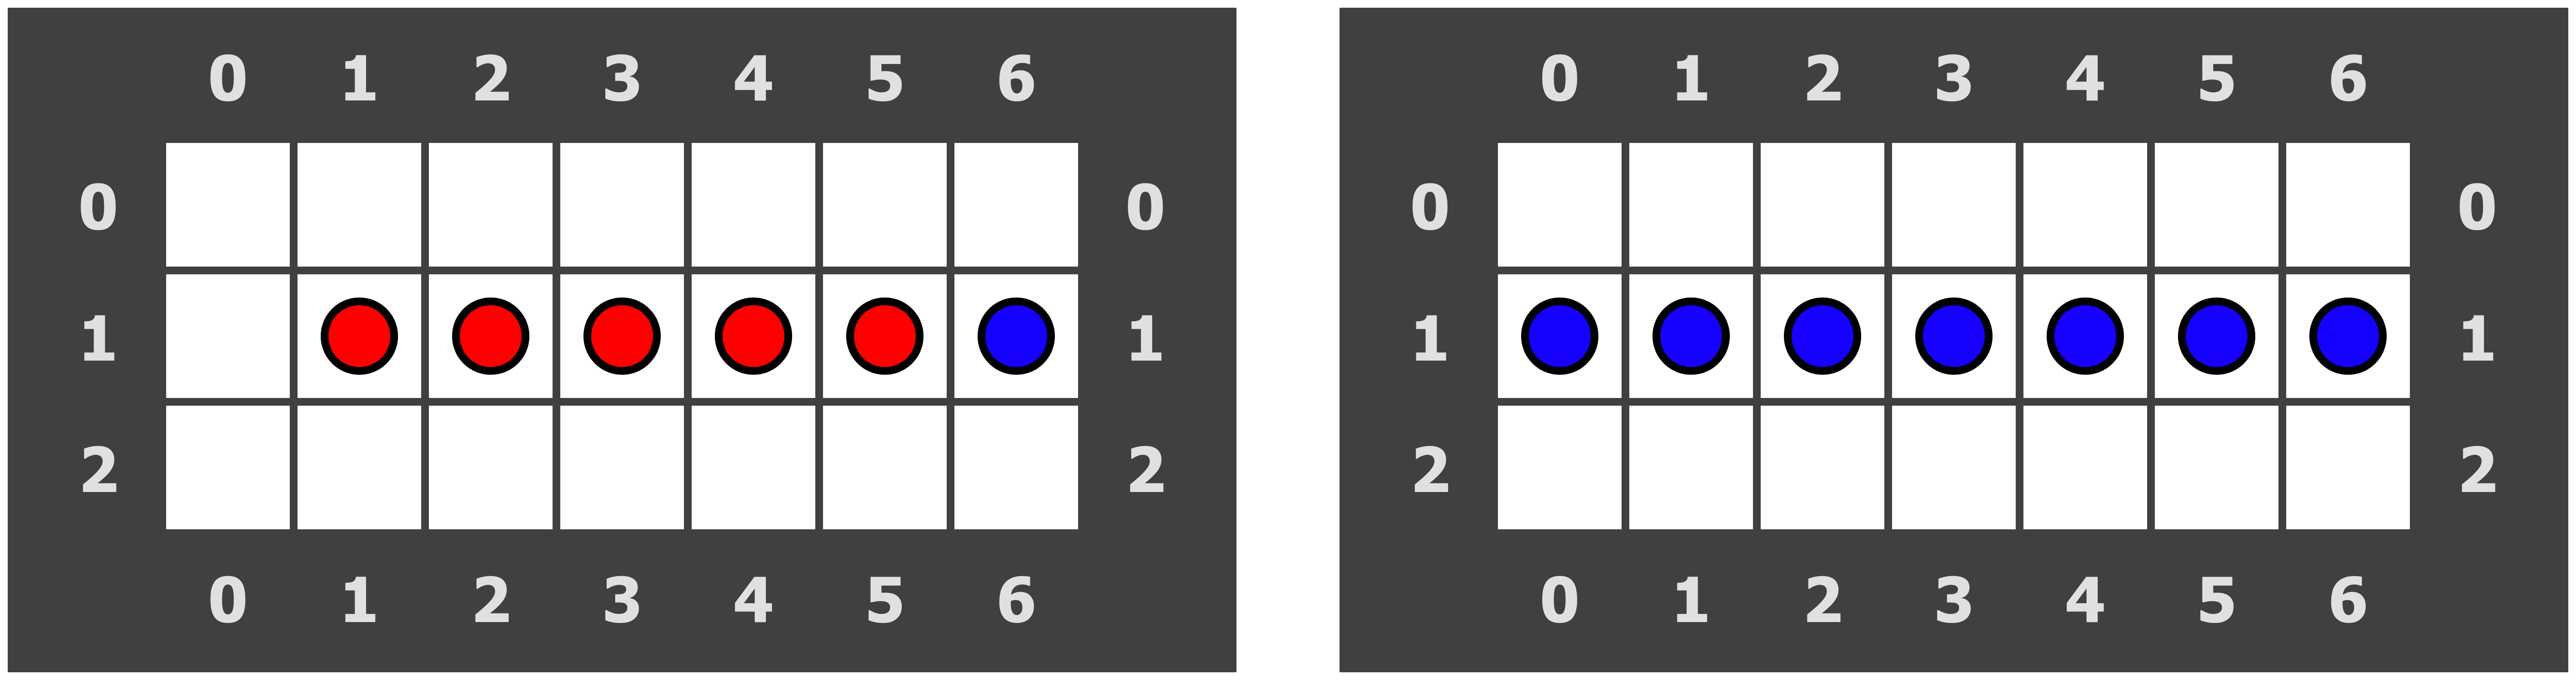
\includegraphics[width=0.6\linewidth]{pics/naive-game-situation}
    \captionof{figure}[Spielfeldsituation 01]{Problematik der naiven Bewertung}
    \label{fig:naivespielfeld01}
\end{minipage}

\subsection{Bestandteile der Heuristik}\label{subsec:bestandteile-der-heuristik}
Wie bereits in der Einleitung dieses Abschnitts begr\"undet, gen\"ugt das reine Abz\"ahlen der Spielsteine nicht aus.
Deshalb setzen wir auf drei unterschiedliche Heuristikbestandteile, um die aktuelle Spielsituation zu bewerten.
Unter diesen drei Ans\"atzen werden die \emph{Mobilit\"at} der Spieler, das \emph{Verh\"altnis der Spielsteine} sowie die aktuelle \emph{Bewertung der Karte} miteinbezogen.
Diese einzelnen Bestandteile sind w\"ahrend des Spiels jedoch nicht immer gleichbedeutend, da zum Beispiel im fr\"uhen Spielverlauf die Mobilit\"at und das Besetzen von wichtigen Feldern von Vorteil ist.
Im sp\"ateren Spielverlauf m\"ussen die einzelnen Bestandteile anders gewertet werden.
Hierbei muss darauf geachtet werden, seine Anzahl an Steinen zu erh\"ohen.

\subsubsection{Gewichtung des Spielfeldes}\label{subsubsec:gewichtung-des-spielfeldes}
Es gibt gewisse Positionen die f\"ur einen Spieler wertvoller sind als andere.
Zu diesen Positionen z\"ahlen unter anderem Kanten und Ecken, da es wesentlich schwieriger, bis garnicht m\"oglich ist, diese einzunehmen.
Eine Ausnahme stellt hier das Einnehmen mithilfe von \"Uberschreib-, bzw.\ Spezialsteine dar.
Insbesondere sind Felder die zwei Felder oder mehr von einem Bonusfeld in direkter Richtung entfernt sind h\"oher gewichtet, da sie die M\"oglichkeit geben einen solchen Bonusstein einzunehmen falls ein Gegner auf ein direktes Nachbarfeld des Spezialfeldes zieht.

\vspace{1em}
\begin{minipage}{\linewidth}
    \centering
    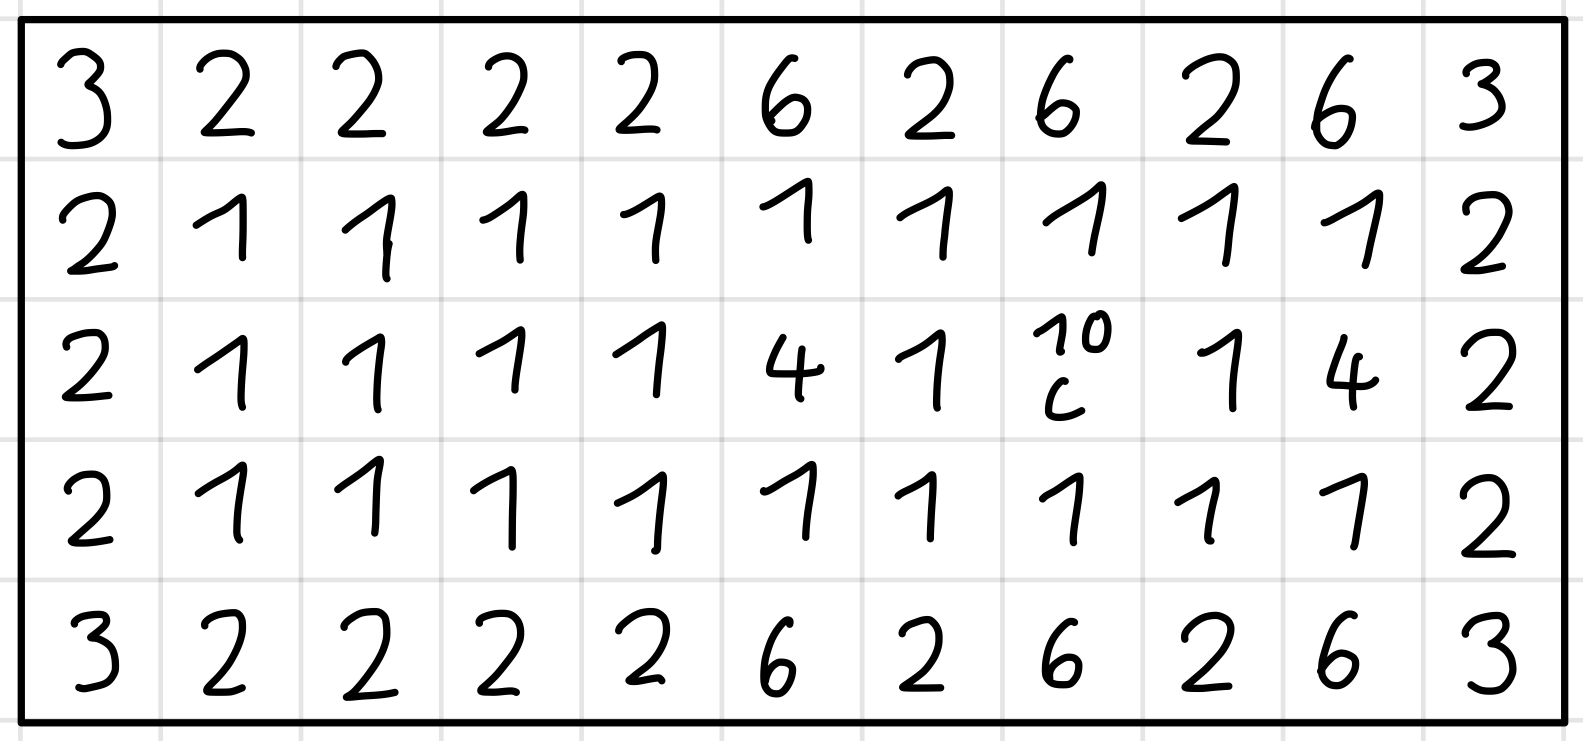
\includegraphics[width=0.5\linewidth]{pics/rating}
    \captionof{figure}[Bewertungsverfahren 01]{Spielfeldpositionen mit Gewichtungen}
    \label{fig:bewertungsverfahren01}
\end{minipage}

Der Score eines Spielers setzt sich dann aus der Summe der belegten Felder mit der entsprechenden Gewichtung zusammen.

Dieses Bewertungsverfahren bietet Vor- und Nachteile.
Positiv daran ist, dass bei Beginn des Spieles jedem Feld eine Gewichtung zugeteilt wird und diese nur noch durch erreichen von Spezialfeldern geringf\"ugig ge\"andert wird.
Negativ ist jedoch, dass dieses Bewertungsverfahren besonders bei gro"sen rechteckigen Spielfeldern mit wenig Spezialfeldern ann\"ahernd wie die naive Variante funktioniert.

\subsubsection{Mobilit\"at}\label{subsubsec:mobilitaet}
Ein weiterer Bestandteil der Analyse besteht darin, Spielsituationen anhand der Beweglichkeit der Spieler einzustufen.
Hierbei wird die Anzahl an Spielz\"ugen eines jeden Spielers bestimmt und miteinander verglichen.
Wie bereits in der Einleitung gezeigt kann ein Spieler seine positive Stellung nur halten, solange er weiterhin spielf\"ahig bleibt.
Aus diesem Grund wird in diesem Ansatz bestimmt wie beweglich ein Spieler gegen\"uber den Anderen ist.

Ein Vorteil dieser Bewertungsmethode besteht darin, dass ein Spieler mit wenig Steinen aber einer hohen Mobilit\"at bei diesem Verfahren nicht negativ bewertet wird.
Ein Problem daran ist jedoch, dass zum Ende des Spieles dieser Ansatz an Relevanz verliert, da zum Schluss nur die Anzahl an eigenen Steinen wichtig ist.

\subsubsection{Spielfeldbelegung}\label{subsubsec:spielfeldbelegung}
Da es besonders gegen Ende des Spiels wichtig ist, viele Steine zu besitzen, muss man dies ebenfalls in die Bewertung miteinbeziehen.
Anstatt aber nur einfach die Anzahl der Spielsteine zu z\"ahlen, wird hier das prozentuale Verh\"altnis gegen\"uber allen existierenden Spielsteinen genommen.

Der Vorteil dieses Verfahrens ist hier, dass man vor allem im sp\"ateren Spielverlauf feststellen kann, wie der aktuelle Stand des Spiels ist und welche Spieler es anzugreifen gilt.
Der Nachteil hierbei ist aber, dass dieses Verfahren im anf\"anglichen und mittleren Spielverlauf nicht aussagekr\"aftig ist.
Allerdings muss man diese Berechnung wie Anfangs erw\"ahnt mit einflie"sen lassen, da man zum Schluss einen Greedyansatz w\"ahlen muss.
Denn letztlich ist f\"ur das Gewinnen des Spieles nur die Anzahl an Spielsteinen von Bedeutung.


\subsection{Algorithmen der Zugauswahl}\label{subsec:algorithmen-der-zugauswahl}
F\"ur einen Computer ist es unm\"oglich den besten Spielzug zu finden, da hier jedes m\"ogliche Spielfeld \"uberpr\"uft werden m\"usste.
Bei einem Spiel wie Schach w\"aren dies circa $10^{120}$ unterschiedliche Spielbrettzust\"ande\citep[vgl.][]{chessBoards}    test\footnote{epubli: Zahlen am Brett, \textit{https://www.schachlich.de/schach-in-zahlen/} (abgerufen am 09.05.2021)}.
Bei ReversiXT liegt die Zahl wesentlich h\"oher, da es zum einen viel gr\"o"sere Karten und zum anderen bis zu 8 Spieler gibt.
Damit ein Computer trotzdem einen guten Zug abliefern kann, ben\"otigt es spezielle Algorithmen.
Ein weit verbreiteter Algorithmus f\"ur Zwei-Personen-Nullsummenspiele\footnote{Duden: Spiel, bei dem die Summe der Einsätze, Verluste und Gewinne gleich null ist} lauter Minimax.

\subsubsection{Minimax Algorithmus}\label{subsubsec:minimax-algorithmus}
Zur Veranschaulichung von Minimax soll ein kurzes Gedankenexperiment (siehe Abbildung~\ref{fig:thought-experiment}) dienen, was auch f\"ur fortlaufende Verbesserungen dienen wird.
Es gibt zwei Personen.
Die eine hat zwei Schubl\"aden A \& B mit je zwei Gegenst\"anden.
Die andere Person darf sich nun einen Schubladen aussuchen, aus dem Sie dann ein Geschenk bekommt.
Nun muss sich der Besitzer dieser Gegenst\"ande aussuchen welches er dem Gl\"ucklichen schenken m\"ochte.
Freilich wird er den Gegenstand w\"ahlen, der f\"ur Ihn am wenigsten Verlust darstellt.
Aus diesen Grund macht es keinen Sinn die Schublade B auszuw\"ahlen, da man hier den Gegenstand f\"ur 1~\euro{} bekommt, andernfalls den f\"ur 20~\euro{}.

\vspace{1em}
\begin{center}
    \begin{tikzpicture}[
        level distance=15mm,
        every node/.style={circle,draw,minimum size=1cm},
        level/.style={sibling distance=60mm/#1}
    ]

        \node{\avlkey{YOU}}
            child {node {\avlkey{A}}
                child {node {\avlkey{30}}}
                child {node {\avlkey{20}}}
            }
            child {node {\avlkey{B}}
                child {node {\avlkey{1}}}
                child {node {\avlkey{120}}}
            }
        ;
    \end{tikzpicture}
    \captionof{figure}[Gedankenexperiment]{Grafik zur Veranschaulichung des Gedankenexperimentes.}
    \label{fig:thought-experiment}
\end{center}

Ein solches Verfahren kann nun genutzt werden um unterschiedliche Spielz\"uge gegeneinander zu vergleichen und den Bestm\"oglichen - unter Ber\"ucksichtung der sp\"ateren Z\"uge des Gegners - auszuw\"ahlen.
Jedoch beinhaltet dieser Algorithmus einen Nachteil - es werden auch Spielz\"uge betrachtet die garnicht in Frage kommen, da ein Spieler diesen Zug niemals w\"ahlen w\"urde.

\subsubsection{Alpha-Beta-Pruning}\label{subsubsec:alpha-beta-pruning}
Dieses Problem kann mithilfe dem Alpha-Beta-Pruning drastisch reduziert werden.
Hierbei werden Hilfsvariablen (alpha und beta) durchgereicht.
Mithilfe dieser Verbesserung werden Zugfolgen, die das Ergebnis nicht beeinflussen, erst garnicht kontrolliert.
Beim Gedankenexperiment muss somit nach dem Gegenstand mit Kosten 1~\euro{} keine weiteren Knoten angeschaut werden, da der Spieler YOU diesen Pfad (im Beispiel die Schublade B) nicht w\"ahlen wird.
Das liegt daran, dass f\"ur ihn die Schublade A wesentlich interessanter ist.
Selbstverst\"andlich nur unter Ber\"ucksichtigung, dass der Andere seinen Verlust minimieren m\"ochte.

\subsubsection{Vergleich der Algorithmen}\label{subsubsec:vergleich-der-algorithmen}
Um die Bedeutung dieser Variante zu verdeutlichen folgt nun ein Vergleich beider Verfahren.
Dabei wurden die selbe Karte mit unterschiedliche Suchbaumtiefen getestet.
Es trat in den Tiefen 3 bis 8 jeweils zwei Spieler gegeneinander an\footnote{Die Suchbaumtiefe 8 wurde auf einem Labor-PC der OTH Regensburg durchgef\"uhrt. N\"ahere Informationen siehe Kapitel~\ref{subsec:technische-daten}}.
Es wurde je einmal der erste Spieler und einmal der zweite Spieler mit Alpha-Beta gestartet.

\vspace{1em}
\begin{minipage}{\linewidth}
    \centering
    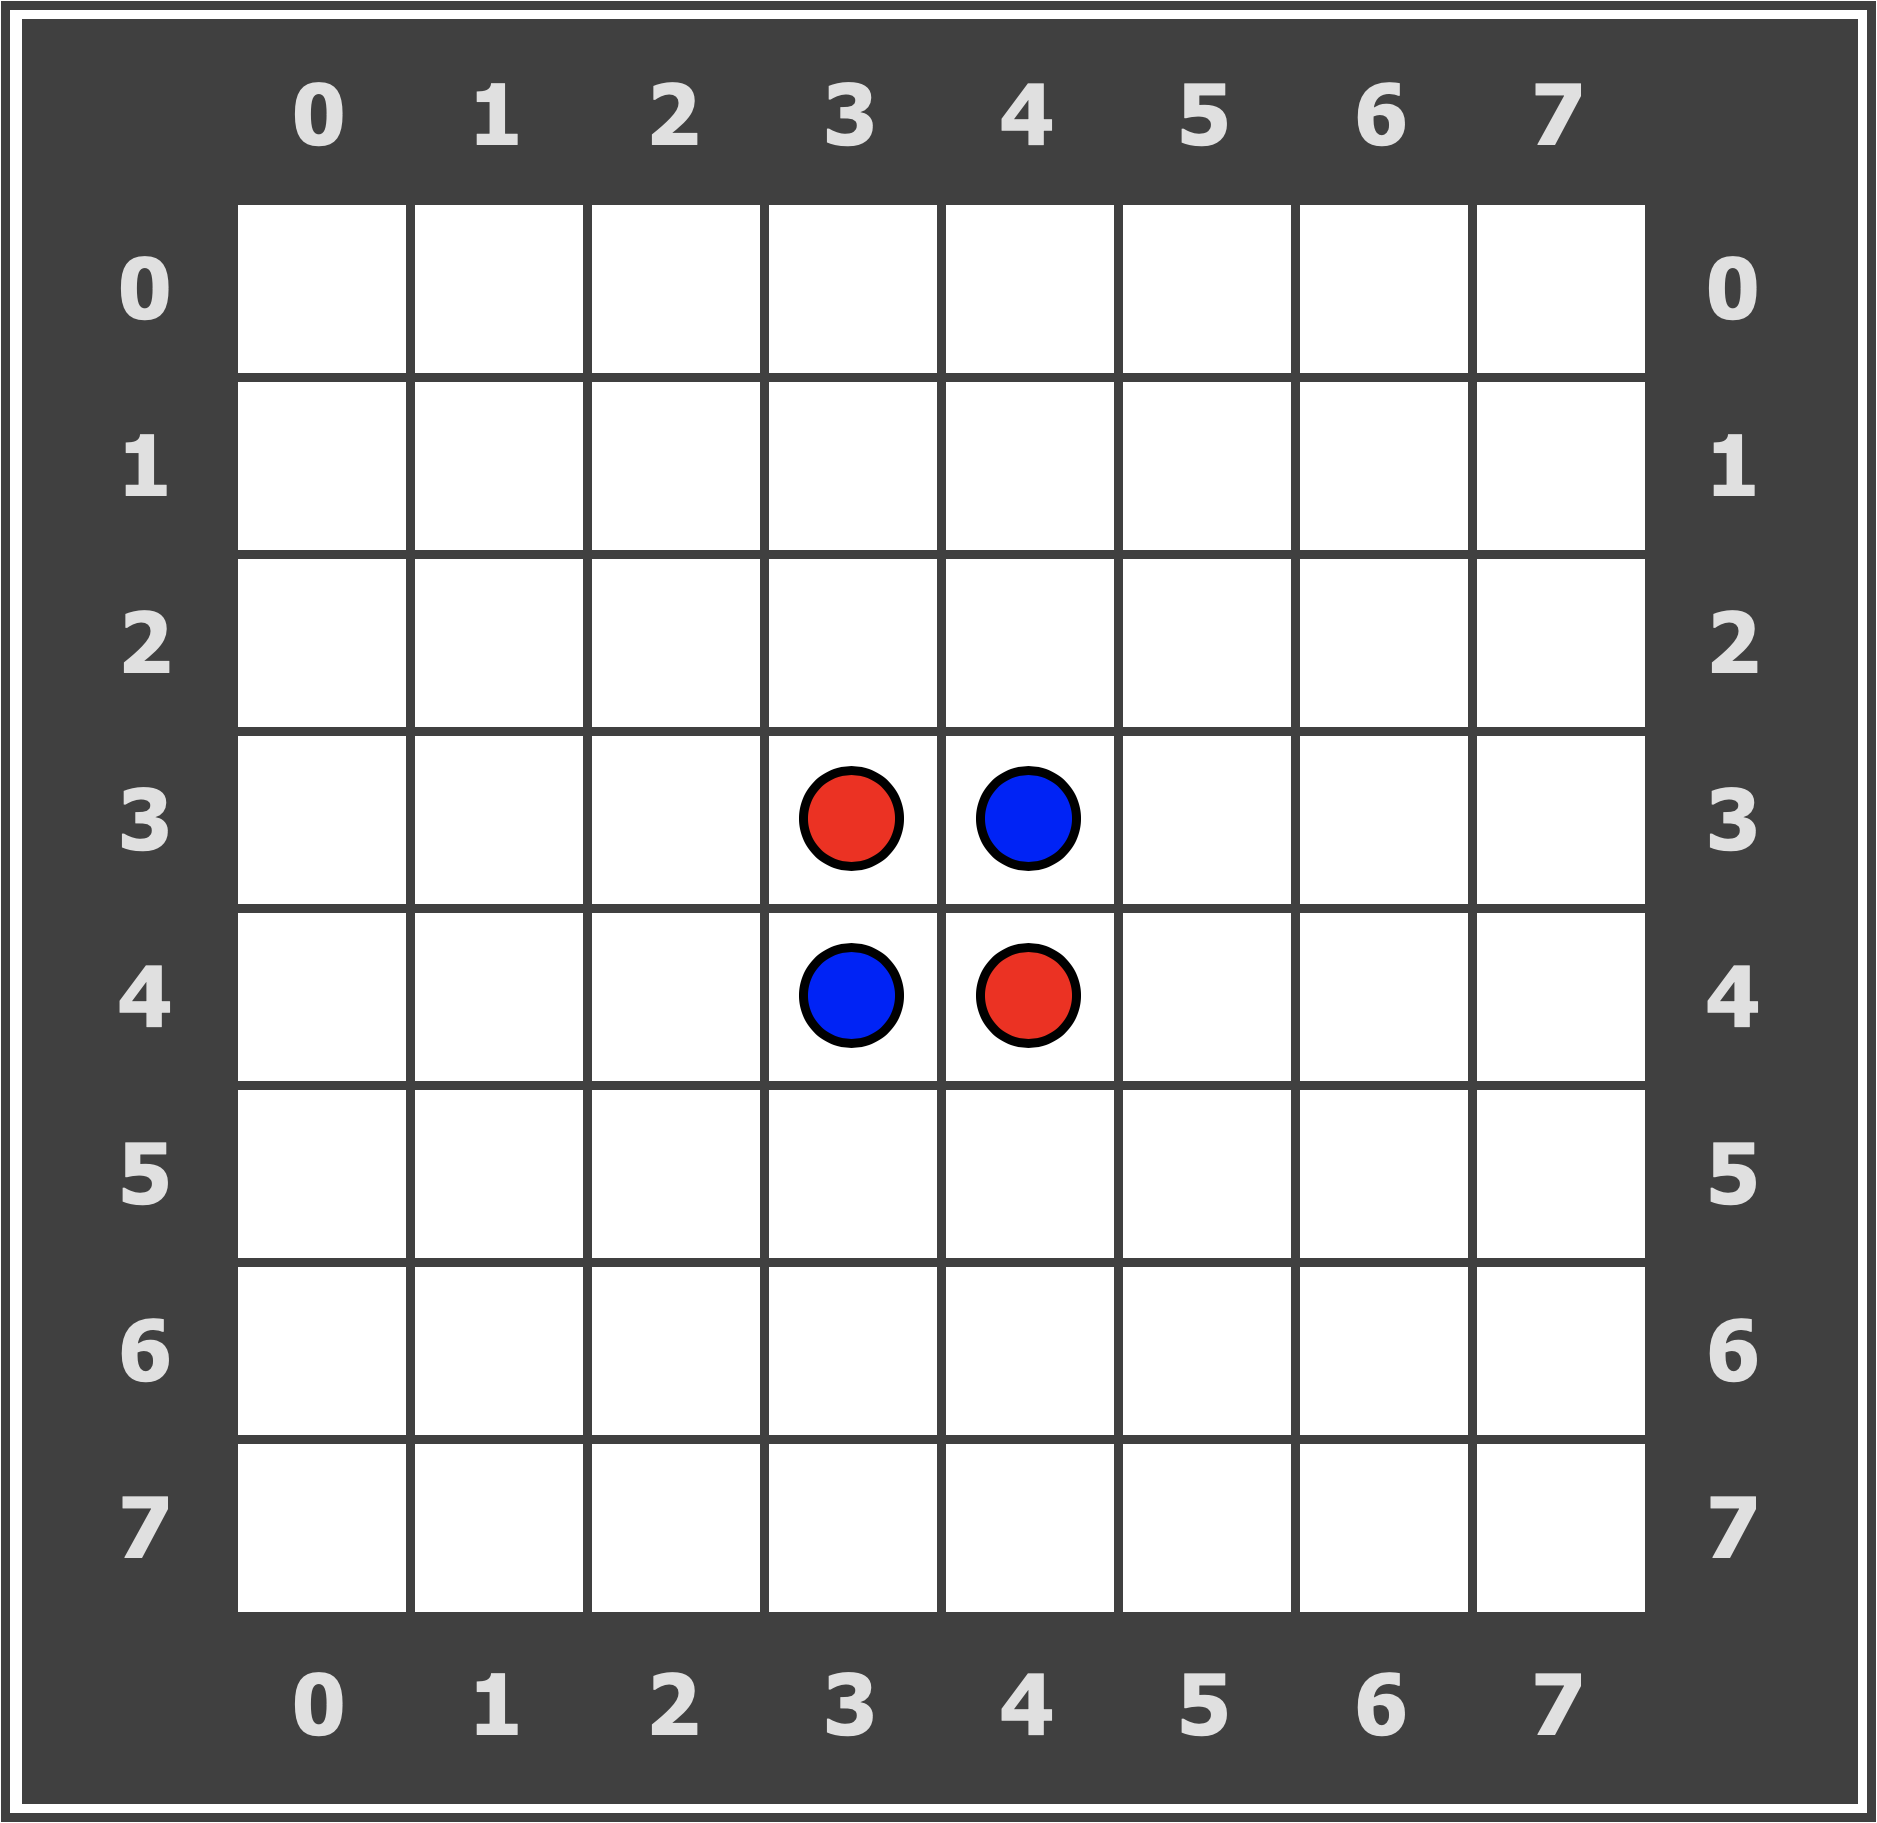
\includegraphics[width=0.3\linewidth]{pics/statistic-map}
    \captionof{figure}[Karte für Statisitk]{Verwendete Karte für den Vergleich von Minimax und Alpha-Beta}
    \label{fig:statistic-map}
\end{minipage}

Wir haben uns aus folgenden Gr\"unden f\"ur die Karte aus Abbildung~\ref{fig:statistic-map} entschieden:
\begin{enumerate}
    \item Es gibt nur zwei Spieler, womit beide Verfahren gegeneinander antreten k\"onnen.
    \item Es gibt keine Spezialsteine, was das Spiel einfacher gestaltet und beim Vergleich der Algorithmen nicht von Bedeutung ist.
    \item Die verwendete Karte ist komplett symmetrisch, wodurch eine Fairness f\"ur beide Spieler garantiert wird.
    \item Es handelt sich um eine relativ kleine Karte, damit die Berechnungen zeitlich einigerma"sen eingegrenzt werden k\"onnen.
\end{enumerate}

\vspace{1em}
\begin{minipage}{\linewidth}
    \centering
    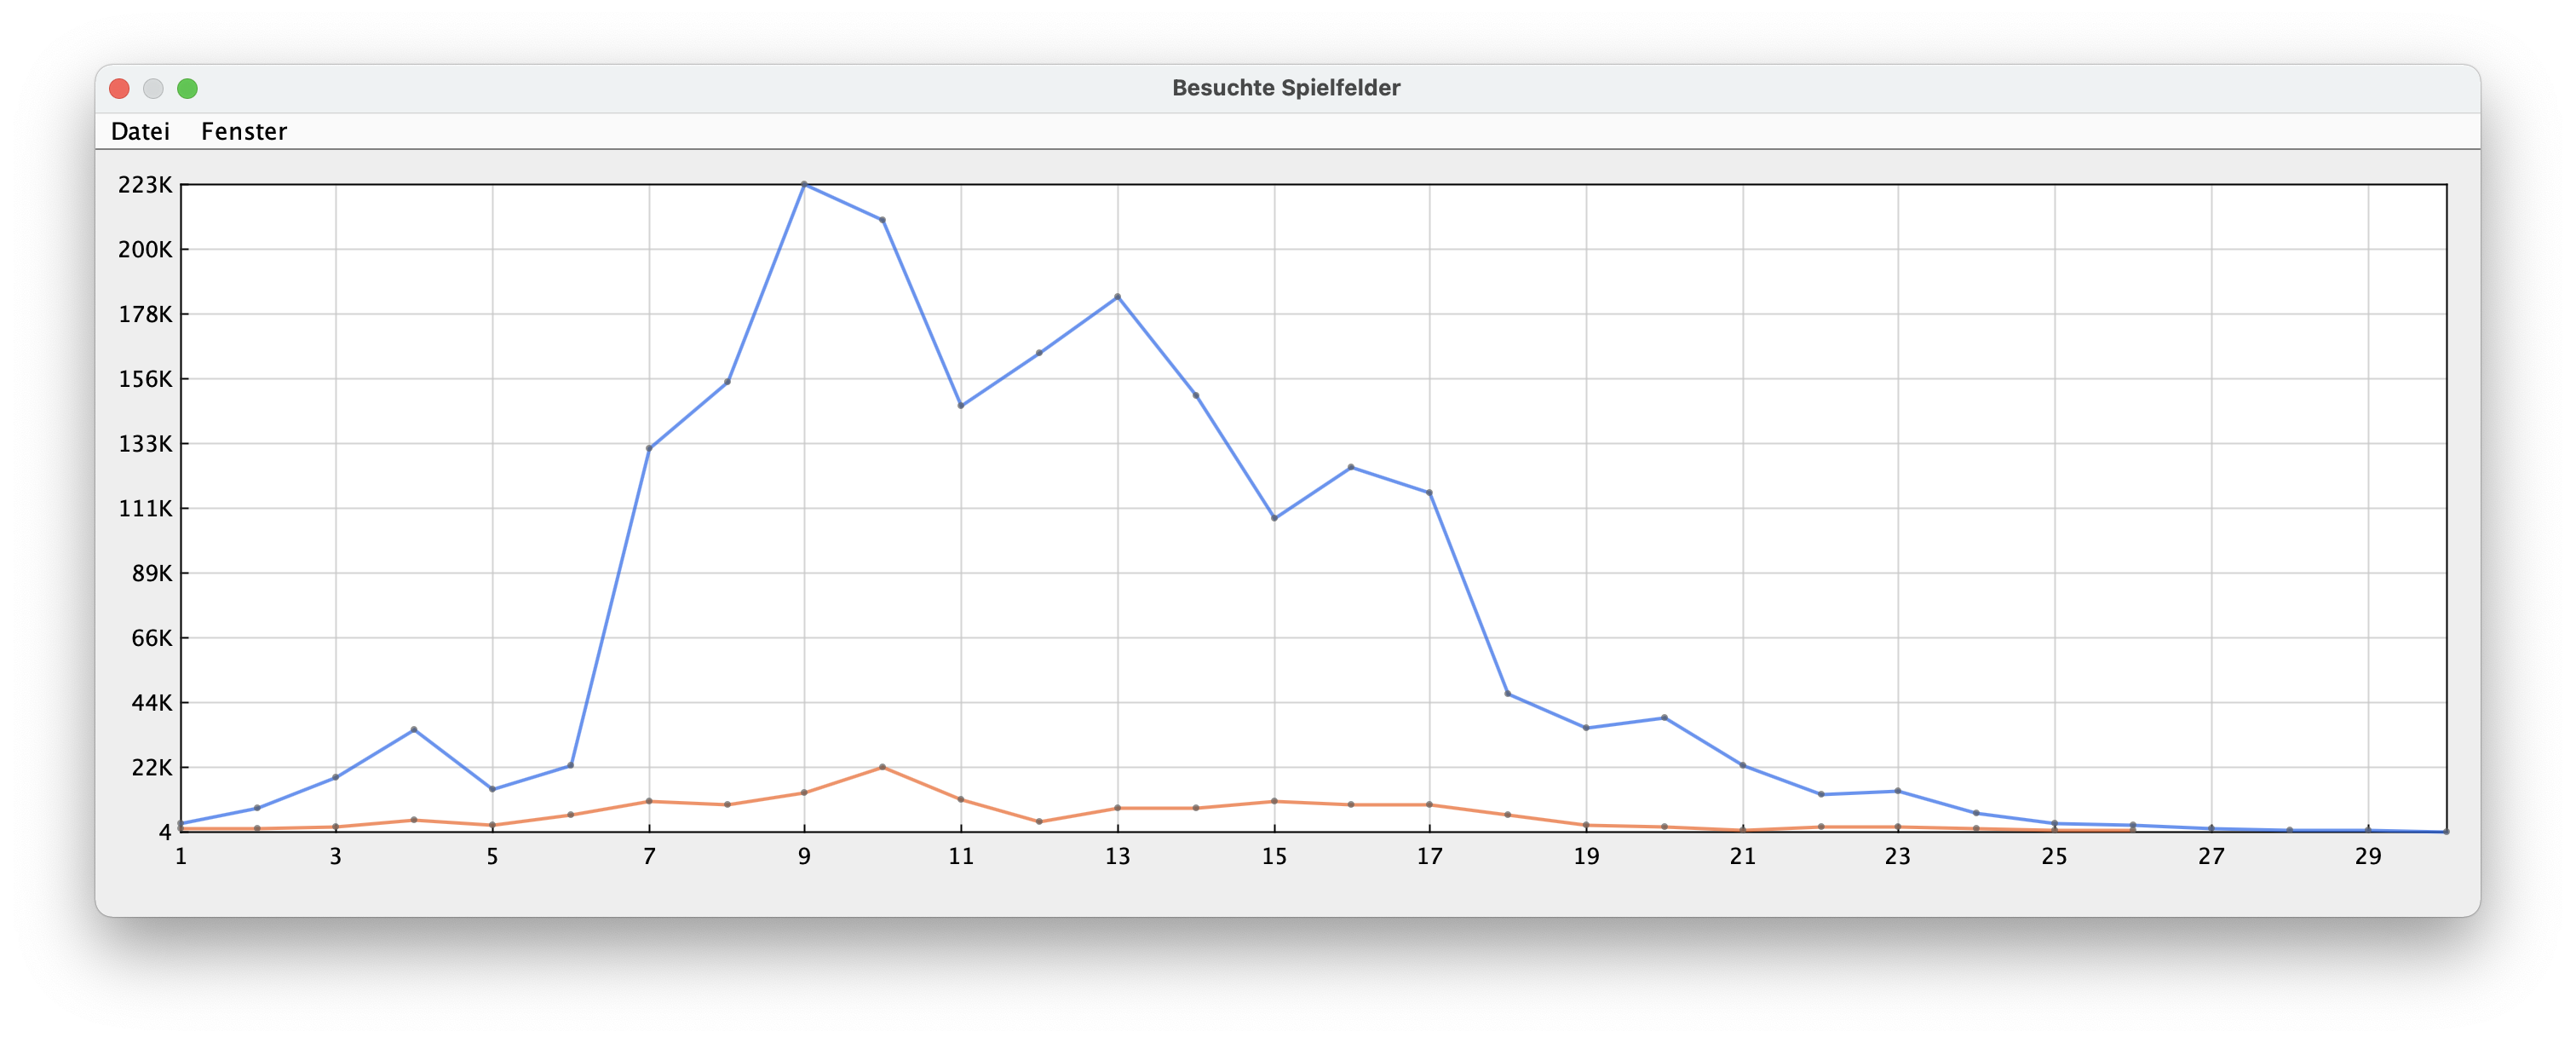
\includegraphics[width=0.9\linewidth]{statistic/Test-D5-01/ST-01-D5-LD}
    \captionof{figure}[Statistik für Tiefe 5]{Diese Statistik wurde bei einem Spiel der Tiefe 5 aufgenommen.}
    \label{fig:statistic-screen}
\end{minipage}

In Abbildung~\ref{fig:statistic-screen} sind sowohl \"uberpr\"ufte Karten ohne Alpha-Beta (blaue Linie), als auch mit Alpha-Beta (orange Linie) zu sehen.
Hierbei ist klar ersichtlich, das Alpha-Beta-Pruning einen enormen Leistungsvorteil liefert.
Der obige Screenshot stammt aus der selbstentwickelten Software GameAnalyzer.
Mehr dazu in Kapitel~\ref{sec:spielanalyse}.

Die Tabelle~\ref{tab:search-depth} liefert eine \"Ubersicht \"uber alle getesteten Suchbaumtiefen dieser Karte.

\vspace{1em}
\begin{table}[!h]
    \centering
    \begin{tabular}{|l|c|c|}
        \hline
        \textbf{Tiefe} & \textbf{Alpha-Beta} & \textbf{Minimax}\\
        \hline
        3 & 1.079,5 & 2.434,5\\
        \hline
        4 & 5.985,5 & 18.417,5\\
        \hline
        5 & 22.653 & 244.854,5\\
        \hline
        6 & 133.657,5 & 1.313.347\\
        \hline
        7 & 419.537 & 28.802.230\\
        \hline
        8 & ? & ?\\
        \hline
    \end{tabular}
    \caption{Besuchte Karten mit den Suchalgorithmen. (Ergebnisse wurden geglättet)}
    \label{tab:search-depth}
\end{table}

Auf den ersten Blick wirken diese Zahlen nun ziemlich bedeutungslos.
Werden Sie jedoch in ein Koordinatensystem (siehe Abbildung~\ref{fig:statistic-graph}) eingetragen und eine Linie eingezeichnet, kann man den Verlauf bei weiteren Suchbaumtiefen beider Algorithmen erahnen.

\vspace{1em}
\begin{minipage}{\linewidth}
    \centering
    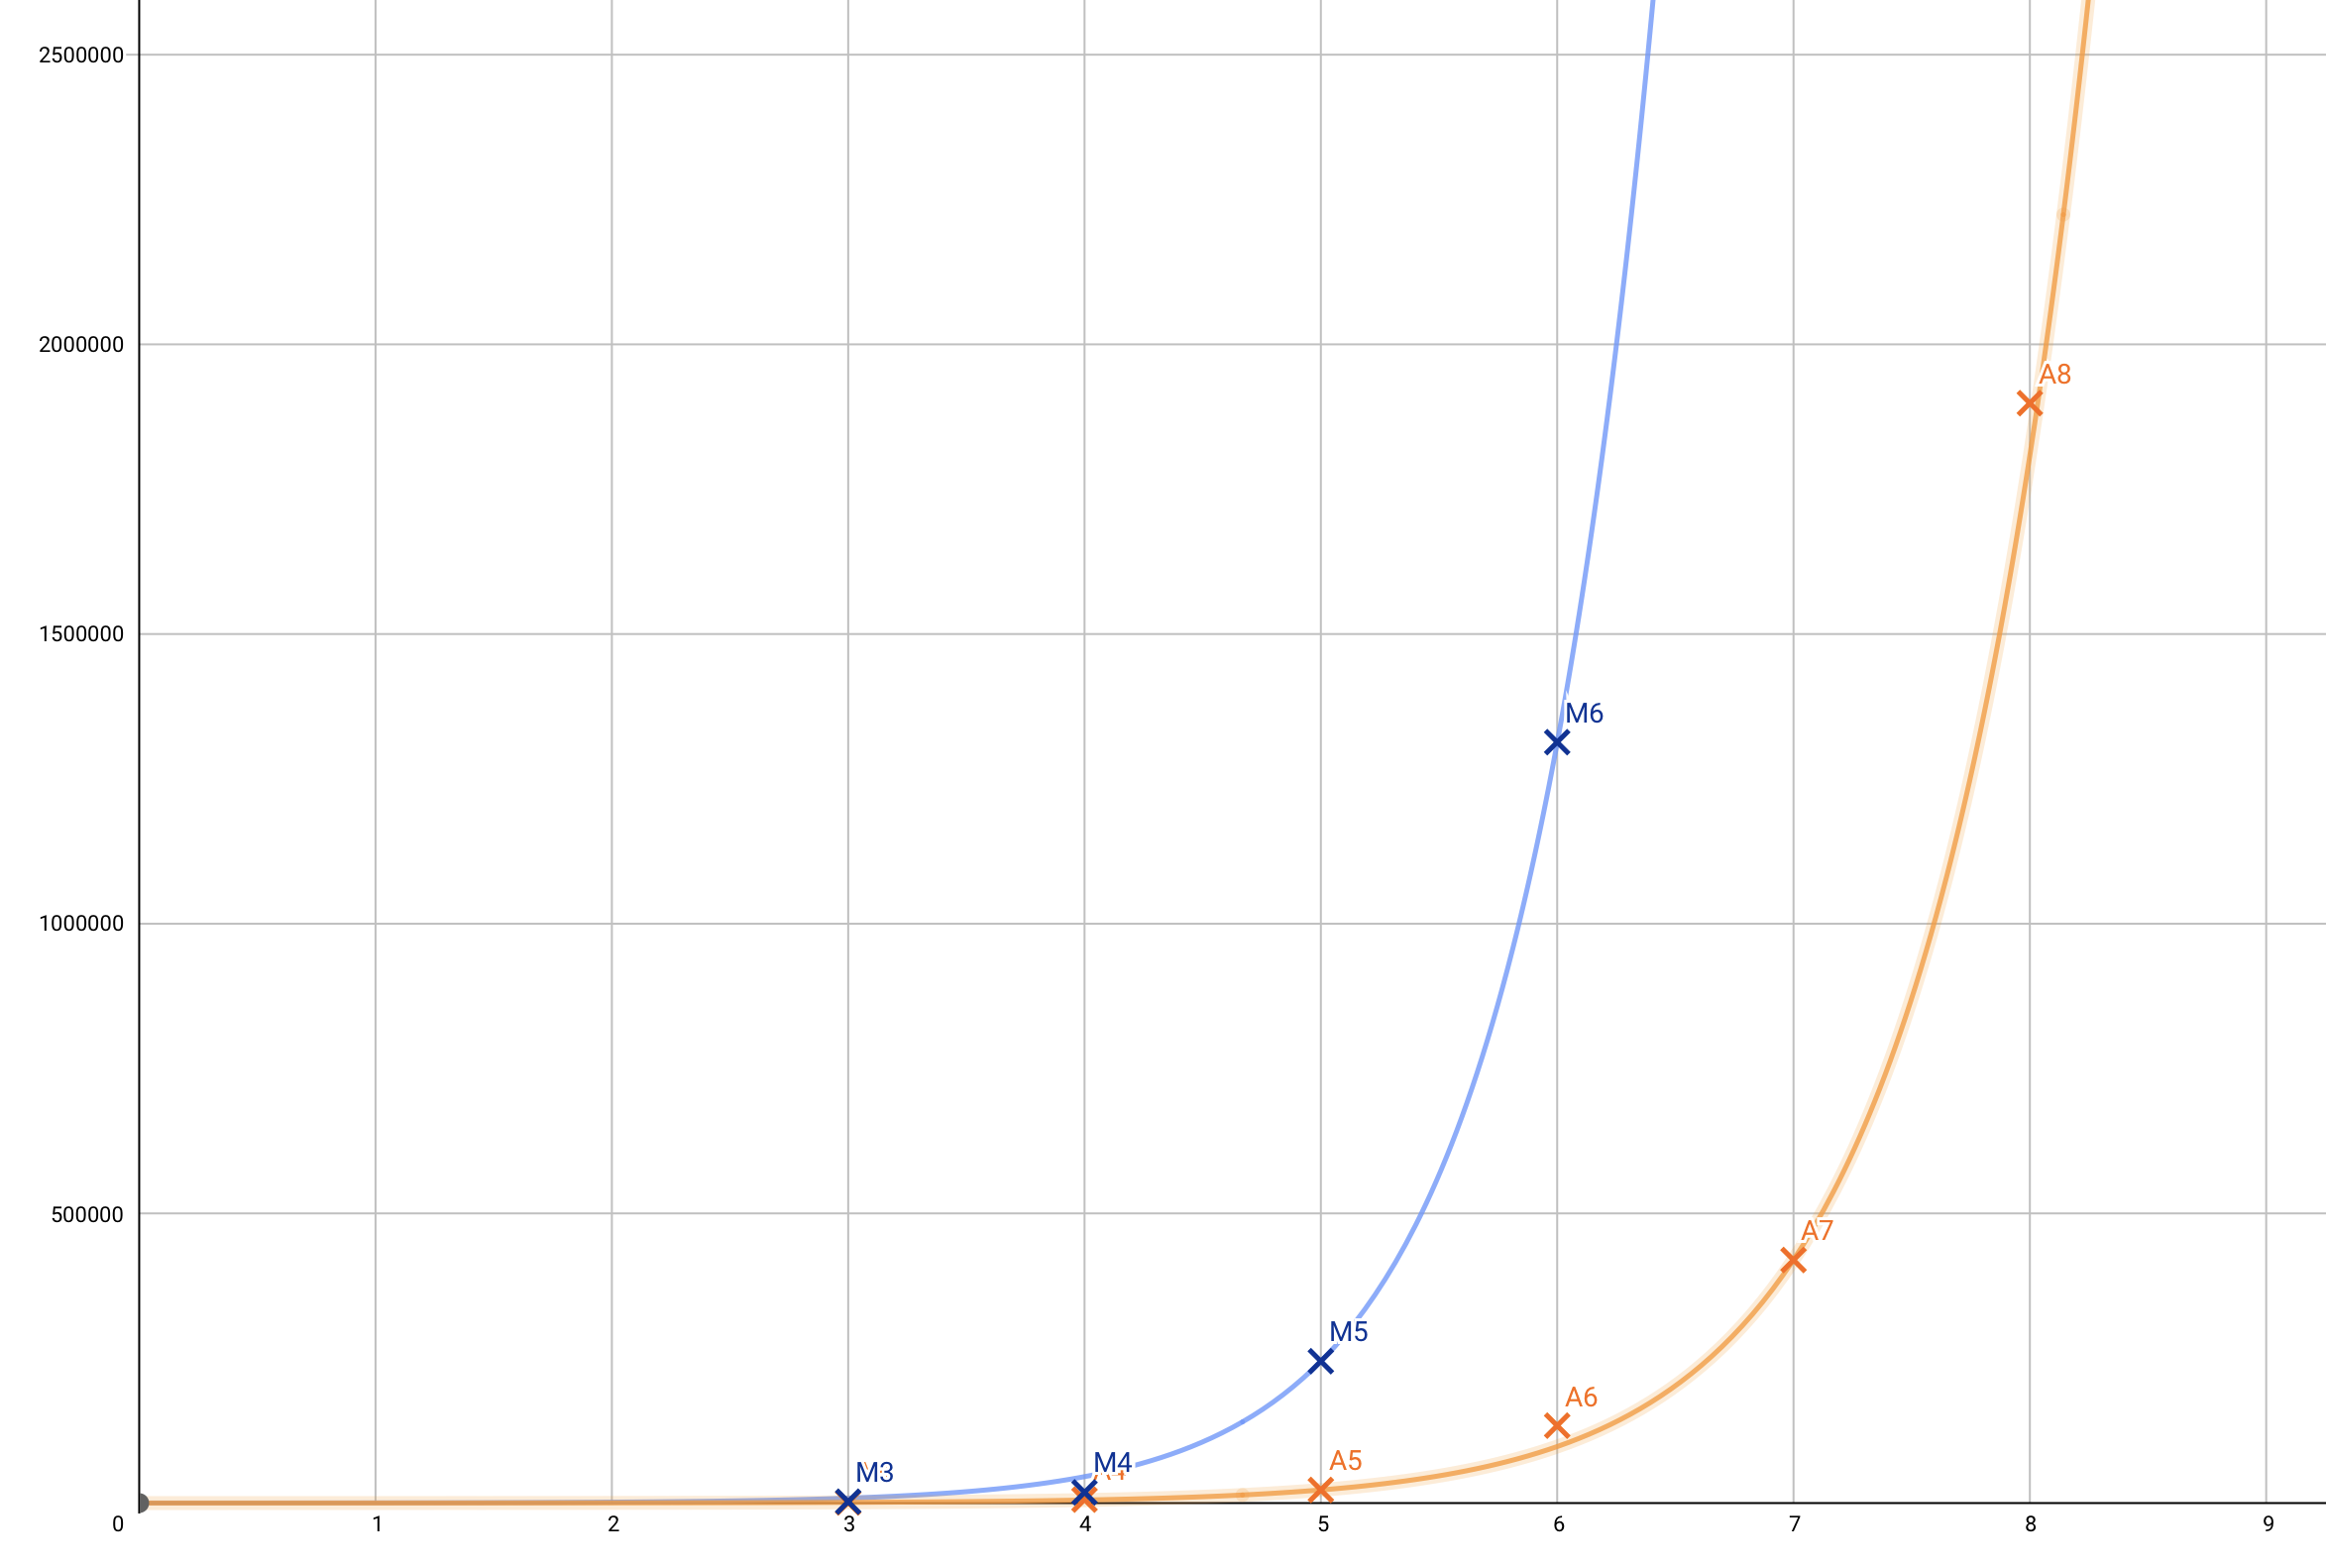
\includegraphics[width=0.7\linewidth]{pics/statistic-graph}
    \captionof{figure}[Suchbaumtiefen in Koordinaten]{Suchbaumtiefen in ein Koordinatensystem eingetragen.}
    \label{fig:statistic-graph}
\end{minipage}

Der Aufwand aller m\"ogliche Spielzust\"ande zu vergleichen w\"achst bei beiden Verfahren exponentiell mit der Anzahl der Suchbaumtiefe.
Jedoch bewirkt des Alpha-Beta-Pruning eine gestauchtere Kurve als der Minimax-Algorithmus ohne Alpha-Beta-Pruning.

Bei gleicher Anzahl an analysierten Felder kann somit mit Alpha-Beta-Pruning weiter in den Suchbaum hineingeschaut und dadurch mehr Z\"uge miteinander verglichen werden.
Das f\"uhrt dazu, dass bei gleichem Zeitaufwand (= gleiche Anzahl an analysierten Spielzust\"anden), das beste Ergebnis einer tieferen Suchbaumebene gefunden wird.

\bigskip
\newpage

% ----------------------------------------------------------------------------------
% Kapitel: Spielanalyse
% ----------------------------------------------------------------------------------
\section{Spielanalyse}\label{sec:spielanalyse}
Um den bestm\"oglichen Client f\"ur ein Spiel zu entwickeln, ist es von besonderer Bedeutung Fehler zu entfernen und stetig die Qualit\"at der Implementierung zu erh\"ohen.
Wir haben bereits zu Beginn festgestellt, dass es nur sehr schwer nachvollziehbar ist, abgeschlossene Spiele zu analysieren.
Wurde man nun durch fehlerhafte Z\"uge disqualifiziert, oder ist der Code bei einer bestimmten Stelle immer abgest\"urzt, war es sehr schwer diese Situation wiederherzustellen.
Zudem sind die aktuellen Informationen \"uber die Heuristik kaum aus gespielten Spielen herauszulesen.
Genau aus diesen Gr\"unden wurde die Software GameAnalyzer entwickelt.

\subsection{Rekonstruktion von Spielen}\label{subsec:rekonstruktion-von-spielen}
Ein wesentlicher Aspekt liegt darin ein gespieltes Spiel Schritt-f\"ur-Schritt nachspielen zu k\"onnen.
Das ist auch der erste wichtige Bestandteil dieser Software.
Wie man in Abbildung~\ref{fig:gameanalyze-start} sehen kann, wird gleich zu Beginn ein Spiel der gew\"ahlten Gruppe eingelesen und alle ausgew\"ahlten Z\"uge nachgeahmt.

\vspace{1em}
\begin{minipage}{\linewidth}
    \centering
    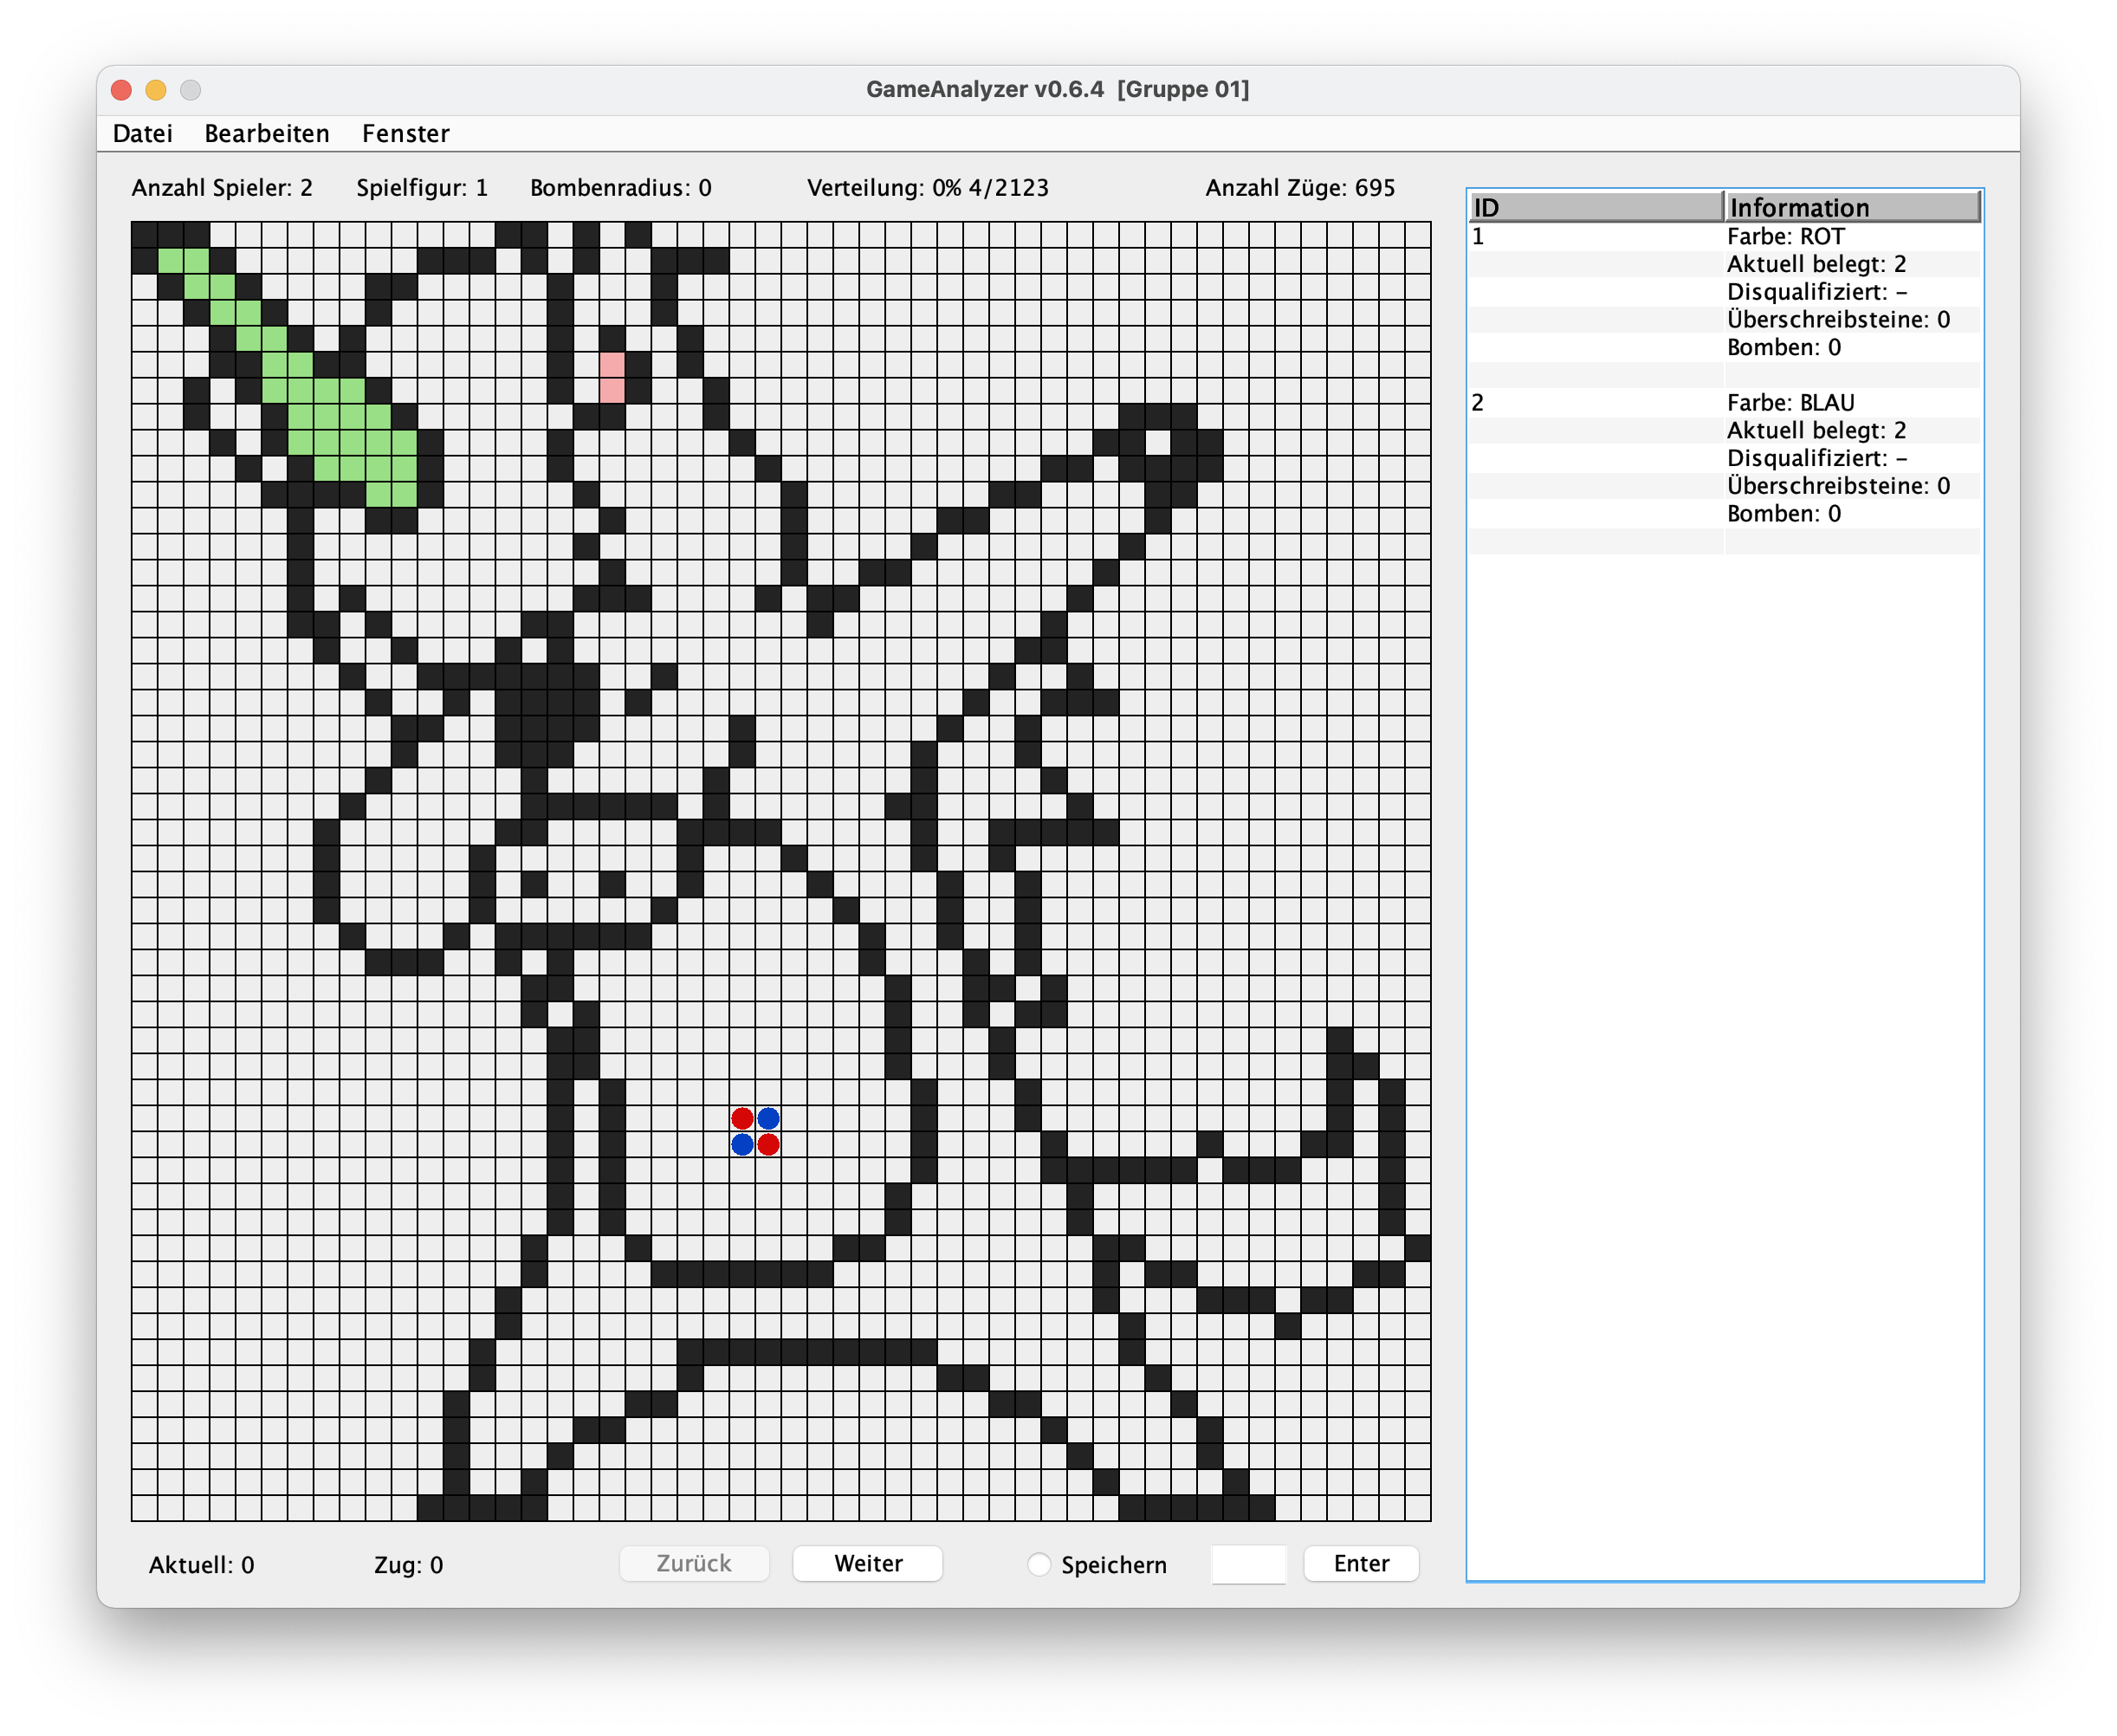
\includegraphics[width=0.7\linewidth]{pics/startscreen}
    \captionof{figure}[Startbildschirm GameAnalyze]{Startbildschirm GameAnalyze nach Auswahl einer Logdatei.}
    \label{fig:gameanalyze-start}
\end{minipage}

Mit den Tasten Weiter und Zur\"uck kann man das Spiel in beide Richtungen durchlaufen.
In der rechten Tabelle werden alle Spieler angezeigt.
Zudem kann man daran erkennen wie viele \"Uberschreibsteine, Bomben bzw.\ Spielsteine sie jeweils aktuell haben.
Ebenfalls ist zu sehen, welche Farbe sie haben und gegebenenfalls wann sie disqualifiziert wurden.
Man erh\"alt zudem Informationen dar\"uber, wie viele Spielz\"uge es gibt und wie viel Prozent an Spielsteinen aktuell belegt sind.
Zudem kann unter Datei $\rightarrow$ Exportieren der aktuelle Stand der Karte exportiert werden, damit die Karte mit dem gew\"unschten Spielstand dann wieder eingelesen werden kann.
Falls Transitionen existieren, k\"onnen diese unter Bearbeiten ein- bzw.\ ausgeschaltet werden.

\subsection{Anzeige erreichbarer Felder}\label{subsec:anzeige-erreichbarer-felder}
Damit keine Spielfelder betrachtet werden m\"ussen die auf dieser Karte garnicht erreichbar sind, haben wir einen MapAnalyzer entwickelt, der zu Beginn des Spieles unerreichbare Positionen aus der Karte herausrechnet.
Welche Felder erreichbar bzw.\ nicht erreichbar sind kann man sich ebenfalls anzeigen lassen.
Dazu geht man auf Fenster $\rightarrow$ Erreichbare Spielfelder.
Nun wird ein Fenster ge\"offnet, wie in Abbildung~\ref{fig:reachable-fields} zu sehen ist.

\vspace{1em}
\begin{minipage}{\linewidth}
    \centering
    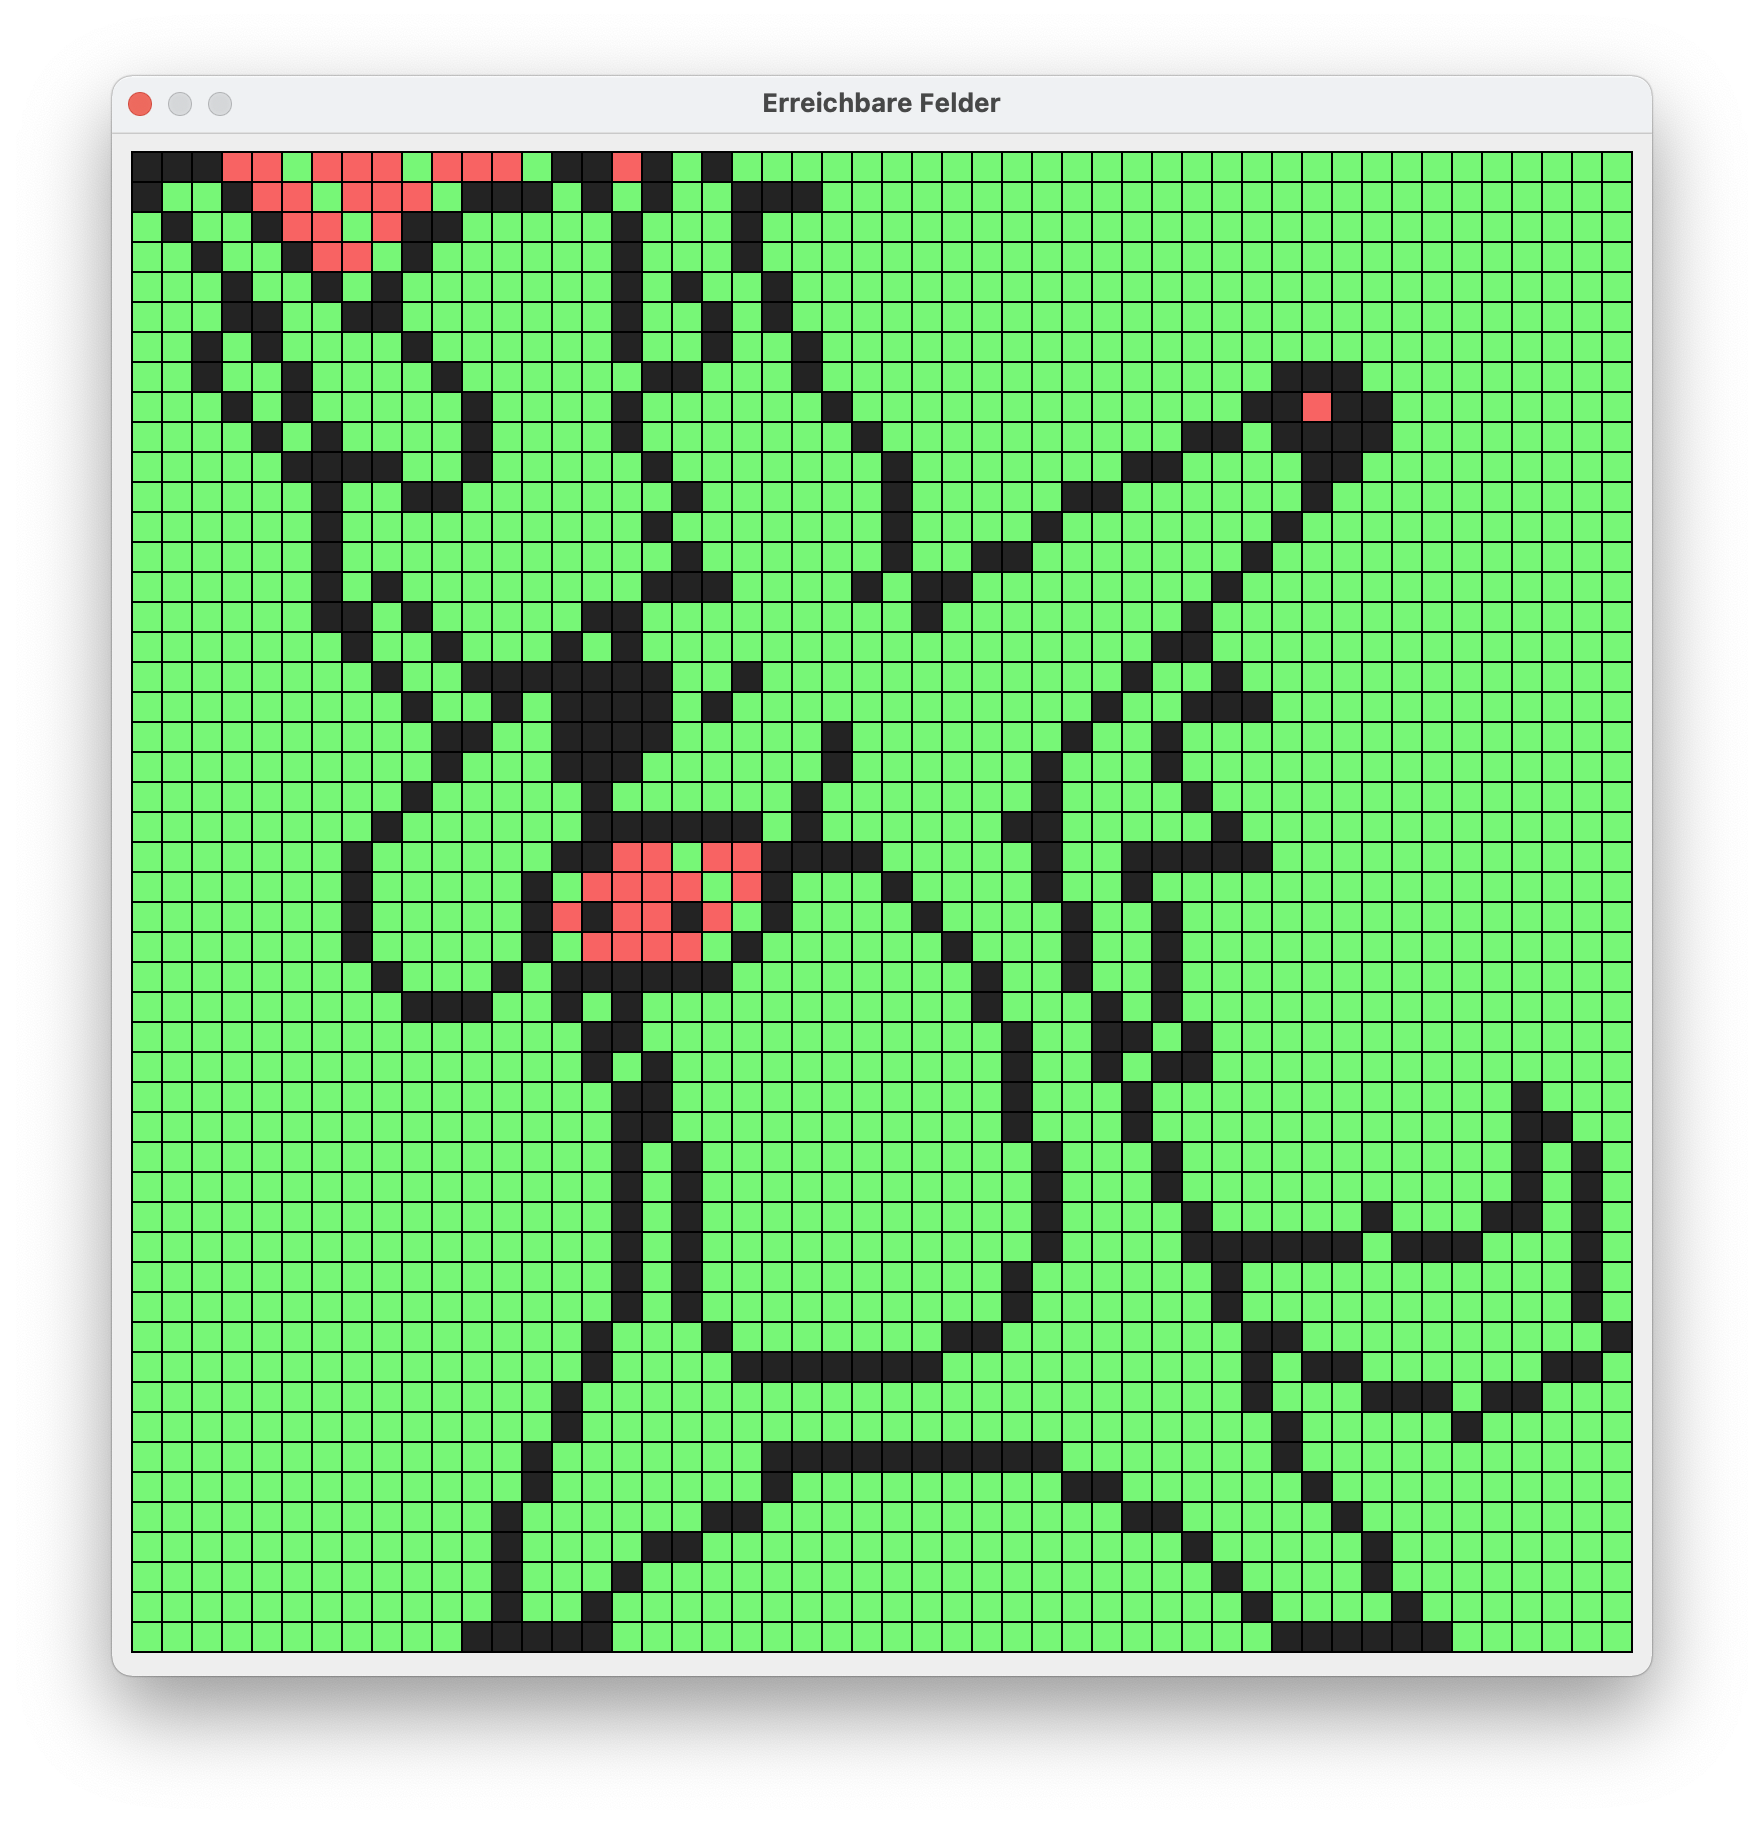
\includegraphics[width=0.7\linewidth]{pics/reachable-fields}
    \captionof{figure}[Anzeige unerreichbarer Felder]{Fenster um unerreichbare Felder anzuzeigen.}
    \label{fig:reachable-fields}
\end{minipage}

Schwarze Felder bedeuten, dass es sich hier um ein Loch handelt und dieses Feld somit generell nicht erreichbar ist.
Gr\"une Felder zeigen die Felder an, die w\"ahrend des Spieles erreichbar sind.
Was jedoch nicht bedeutet, dass sie erreicht werden m\"ussen.
Rote Felder symbolisieren, dass diese Felder w\"ahrend des gesamten Spieles definitiv nicht erreicht werden k\"onnen.

\subsection{Anzeigen detaillierter Statistiken}\label{subsec:anzeigen-detaillierter-statistiken}
Unter Fenster kann man sich die unterschiedlichen Statistiken anzeigen lassen.
Wie Sie in Abbildung~\ref{fig:heuristic} sehen k\"onnen, wird damit der gesamte Zustand eines Spielers w\"ahrend des Spieles angezeigt.
Dabei wird immer die aktuelle Implementierung verwendet.

\vspace{1em}
\begin{minipage}{\linewidth}
    \centering
    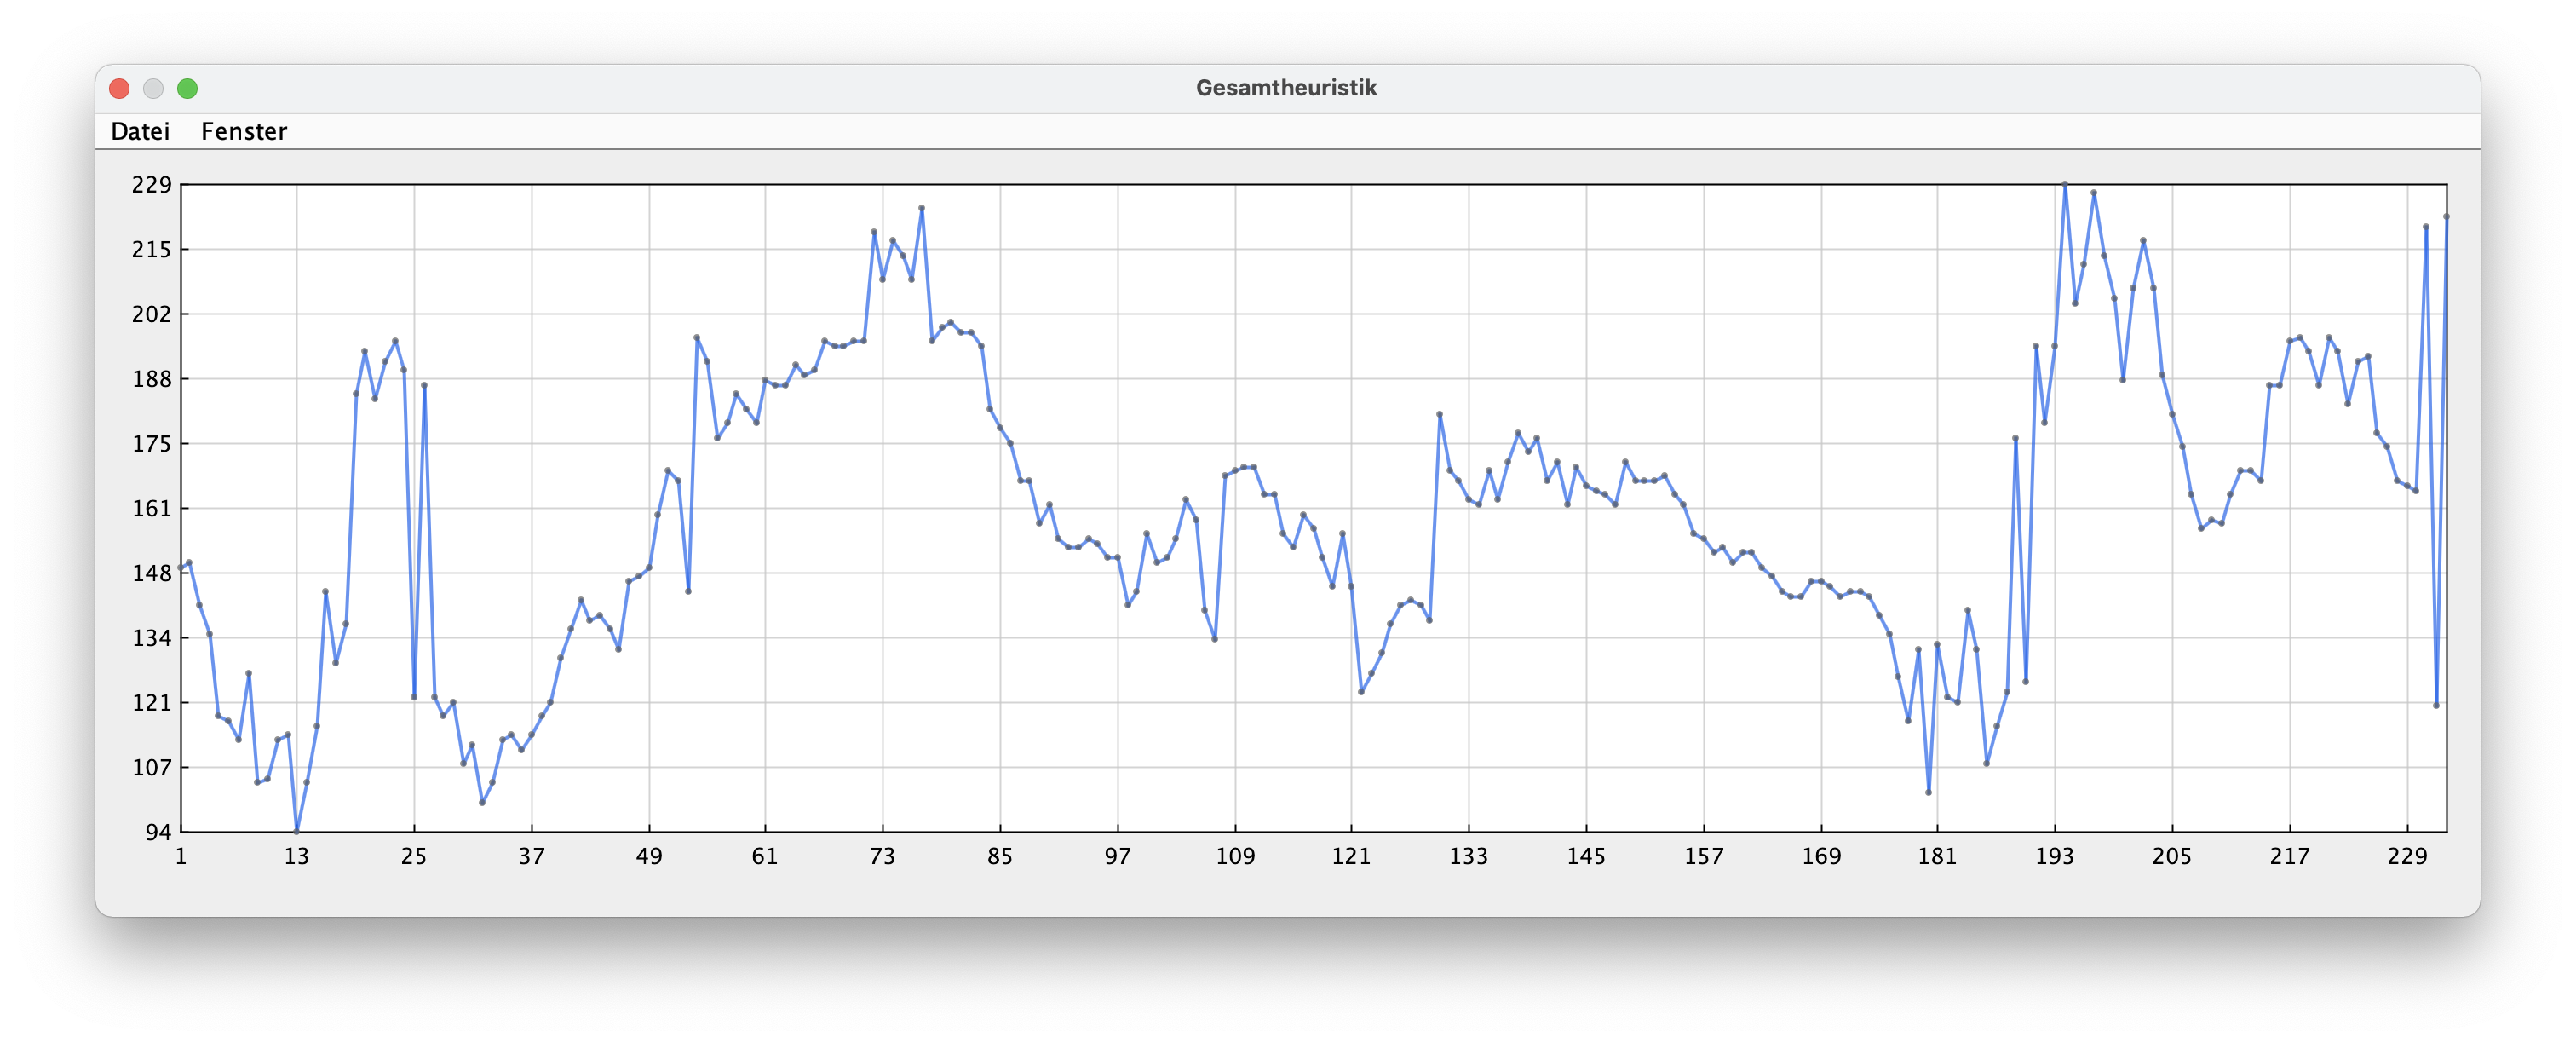
\includegraphics[width=0.8\linewidth]{pics/heuristic}
    \captionof{figure}[Grafik der Heuristik]{Fenster um aktuelle Heuristik anzuzeigen.}
    \label{fig:heuristic}
\end{minipage}

M\"ochte man Zust\"ande der Heuristik f\"ur sp\"ater speichern, kann man sich diese selbstverst\"andlich exportieren lassen und mit Grafiken in der Zukunft vergleichen.
Ein solcher Vergleich kann nat\"urlich auch dazu genutzt werden, um unterschiedliche Spieler bzw.\ Varianten miteinander in Relation zu setzen.
Dies haben sie bereits in Kapitel~\ref{subsubsec:vergleich-der-algorithmen} gesehen.

\subsection{Nutzen der Spielanalyse}\label{subsec:nutzen-der-spielanalyse}
Die Entwicklung der Spielanalyse war ein ziemlich zeit-kostenintensiver Prozess.
Es werden des \"Ofteren Spiele gegen andere Teams \"uber die Plattform Matchpoint gespielt.
Im Anschluss werden die Logdateien an die Gruppen verteilt, damit man eventuelle Abst\"urze finden oder auch generell den Spielverlauf anzeigen und verbessern kann.
Ein solches Turnier liefert gerne mal mehrere Hunderte Logfiles, die man sich am Besten alle genaustens anschauen sollte.
Diese Software tr\"agt wesentlich dazu bei, dass das f\"ur uns in \"uberschaubarer Zeit und noch dazu sehr detailliert m\"oglich ist.


\bigskip
\newpage

% ----------------------------------------------------------------------------------
% Kapitel: Fazit
% ----------------------------------------------------------------------------------
\section{Fazit}\label{sec:fazit}
Die Vorfreude auf dieses Wahlpflichtmodul war bereits vor dem Vorlesungsstart sehr gro"s.
Vor allem der Gedanke ein eigenes Projekt von Anfang bis Ende zu planen, entwickeln, testen und lauff\"ahig spielen zu sehen trug ma"sgeblich dazu bei.

ZOCK ist ein sehr zeitintensives, jedoch auch unglaublich spannendes Modul.
Man sammelt hier in allen erdenklichen Bereichen neue Erfahrungen, wie zum Beispiel die Planung eines Softwareprojekts, verfassen eines wissenschaftlichen Berichtes, Entwicklung von Algorithmen sowie die Zusammenarbeit in einem Team.
Vor allem, wenn gravierende Fehler entstehen oder der Client unerwartet x-mal disqualifiert wird, merkt man, dass man ein Team ist und gemeinsam die Probleme angehen und beheben muss.
Hier wird nicht nur Erfahrung im Bereich Softwareentwicklung, sondern auch im Zwischenmenschlichen gesammelt.

Die einzelnen Beteiligten, haben eine so gro"se Begeisterung f\"ur diesen Kurs entwickelt, dass nicht nur die notwendigen Aufgaben erf\"ullt wurden, sondern viele weitere Ideen in dieses Projekt geflossen sind.
Es existiert aufgrund dieser Freude an ZOCK eine neue M\"oglichkeit, Spiele und Karten detaillierter zu analysieren.
Diese M\"oglichkeit entstand bez\"uglich der Entwicklung des MapAnalyzers, wodurch erreichbare Felder erkannt werden.
Der GameAnalyzer steht in Zukunft anderen Gruppen zu Verf\"ugung, damit diese die gleichen Vorteile haben, um Spiele nachtr\"aglich zu analysieren, exportieren, modifizieren und Statistiken aufzurufen.
Es gibt zudem eine intelligente Zugsortierung, die die Probleme der naiven Zugsortierung behebt und damit extreme Leistungsopimierungen bietet.

Vor allem aber am eigentlichen Entwicklungsfortschritt sieht man, dass man Projekte nur sehr schwer durchplanen kann und man des \"Ofteren ein Refactoring betreiben, neuere Erkenntnisse einarbeiten oder komplett andere Funktionalit\"aten hinzuf\"ugen muss.
Durch diese stetigen Ver\"anderungen und Anpassungen hat das Team wertvolle Erfahrungen bez\"uglich Softwareentwicklung und Softwareplanung sammeln k\"onnen.
Besonders hervorzuheben ist, dass alle vorherigen Module in diesem Kurs Verwendung finden, sei es PG1 oder PG2 um ordentlichen Code zu produzieren, oder AD um leistungsstarke Algorithmen zu verstehen und zu entwickeln.

Im Allgemeinen ist der Aufbau dieser Lehrveranstaltung sehr gut durchdacht und strukturiert aufgebaut.
Der Professor fordert sehr viel von seinen Studenten, ist daf\"ur aber auch bereit sehr viel zu opfern.
Man erh\"alt einen fundierten Umfang \"uber die Entwicklung einer k\"unstlichen Intelligenz und wie diese schrittweise verbessert wird.
Man lernt zudem mit R\"uckschl\"agen umzugehen, da man des \"Ofteren an der Spitze kratzen kann und kurze Zeit sp\"ater wieder von anderen Clients vernichtend geschlagen wird.
Auf all diese Erfahrungen m\"ochte niemand aus dem Team verzichten.
Die Erwartungen waren gro"s, welche jedoch weit \"uberstiegen wurden.
Wer sich dieses Modul und den Arbeitsaufwand zutraut, sollte es definitiv belegen.


\bigskip
\newpage

% ----------------------------------------------------------------------------------
% Kapitel: Anhang
% ----------------------------------------------------------------------------------
\section{Anhang}\label{sec:anhang}
\begin{minipage}{\linewidth}
    \centering
    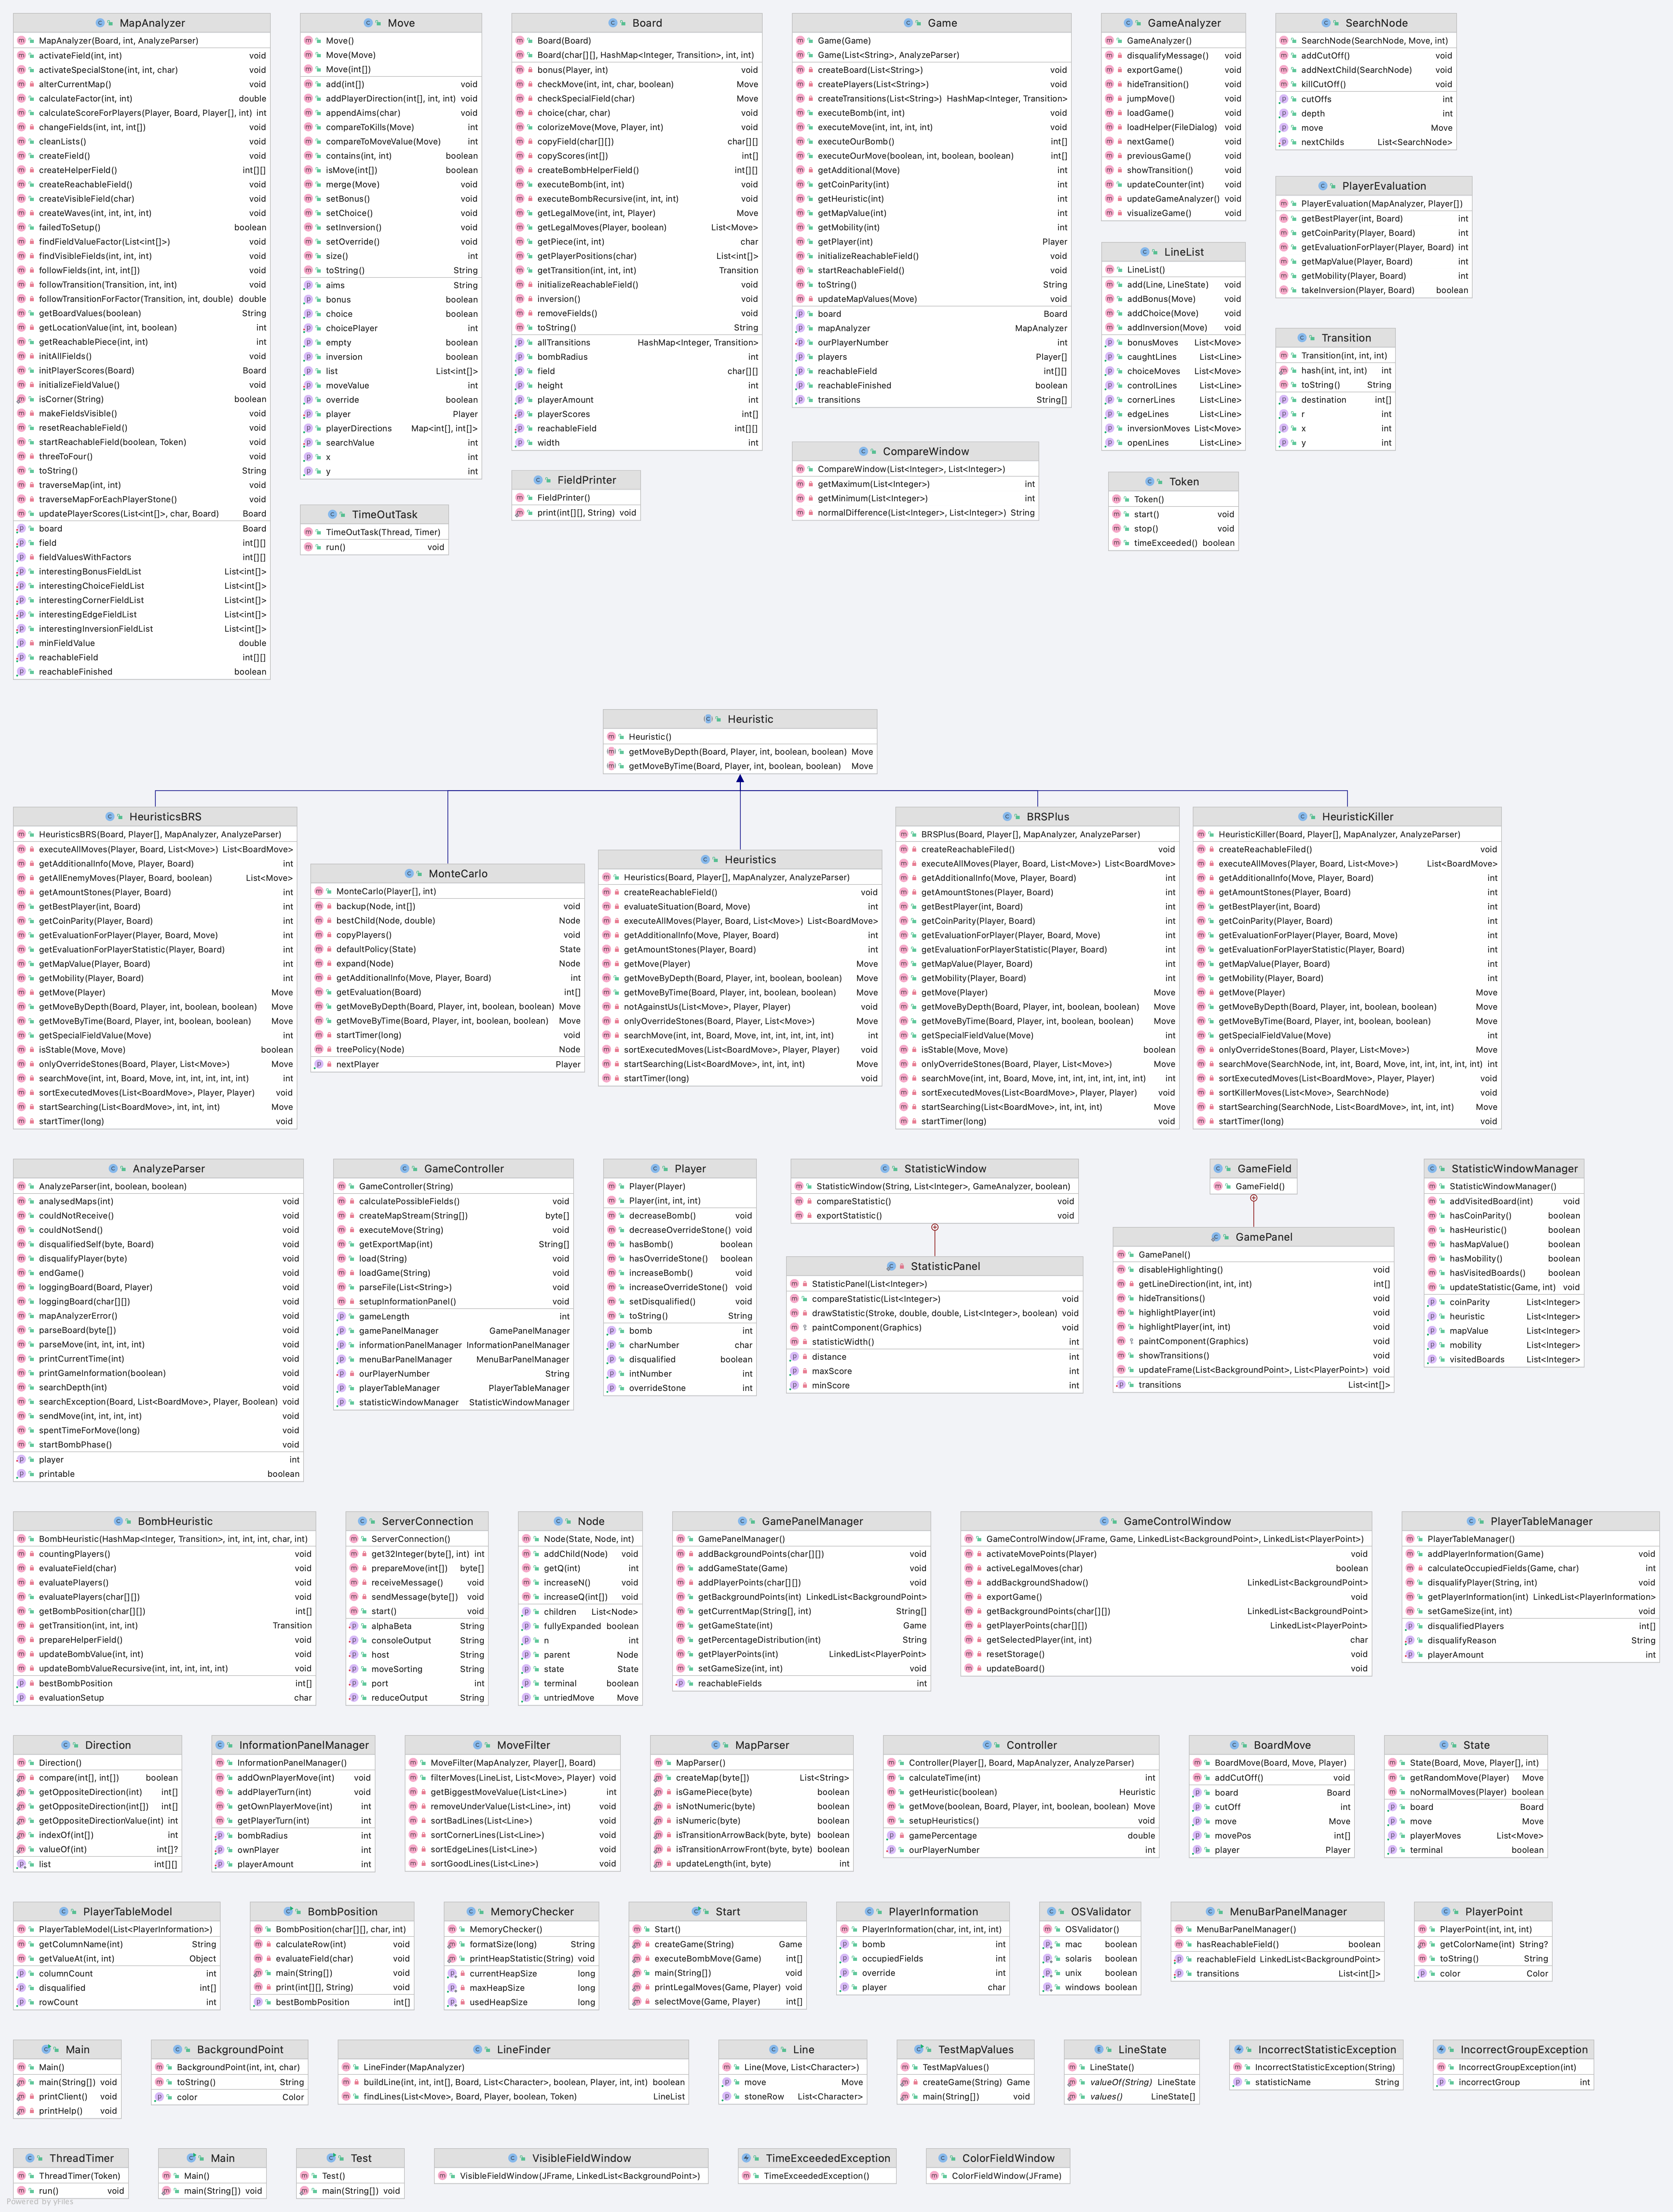
\includegraphics[width=0.95\linewidth]{pics/uml-diagrams}
    \captionof{figure}[UML-Diagramm]{UML Klassendiagramm des Projektes.}
    \label{fig:uml-diagram}
\end{minipage}


\bigskip
\newpage

\end{document}
